\documentclass[12pt]{article}
%pdflatex --shell-escape AMASeriesFEDS.tex 

% \usepackage[authoryear]{natbib}
% \usepackage{amsmath}
% \usepackage{hyperref}
% \usepackage{hyperref}
% \usepackage{geometry}
\usepackage[margin=1.0in]{geometry}
% \usepackage{graphicx}
% \usepackage{amsfonts}
\usepackage{draftwatermark}

\input{../../paperProduction/occBind/docs/AMArepresentationNewCmds}



\author{Gary S. Anderson\thanks{The analysis and conclusions set forth are those of the author and do not indicate concurrence by other members of the research staff or the Board of Governors. I would like to thank Luca Guerrieri, Christopher Gust, Hess Chung, Benjamin Johannsen  and Robert Tetlow for their comments and suggestions.  And special thanks to Luca Guerrieri for first noticing that the series representation formulation could lead to an error bound for model solutions. Any remaining errors are mine alone.}}

\title{A New Series Representation for 
  Nonlinear Dynamic Stochastic Model Solutions: 
  Error Bounds and a New Solution Algorithm} %(Better?, Coherent? Comprehensive? General? )

\date{\today: \currenttime}
\begin{document}
%\SetWatermarkText{preliminary}
%\SetWatermarkScale{2}



\maketitle

\begin{abstract}
This paper investigates the solution of discrete time  dynamic stochastic
infinite-horizon economies with bounded-time-invariant solutions.
The paper provides formulae for evaluating the accuracy of decision rules
approximately satisfying the system of first-order conditions and presents
an algorithm that robustly improves the accuracy of proposed solutions.
The error bounds apply for assessing the accuracy of any proposed bounded time invariant decision rule, regardless of the source.

A straightforward applications of a  new series representation
for bounded discrete time series, appropriate for
a very broad class of dynamic stochastic models, delivers these results.
% This error bound calculation accounts for the impact of errors in any of the equations in the system.
Using the series representation, the paper 
augments a traditional solution strategty with an additional set of
constraints thereby
enhancing algorithm robustness and improving accuracy.
The technique can readily accommodate models with multiple invariant spaces
and, like the error bound formula,  is appropriate
for models with occasionally binding constraints and regime switching. 





The  paper uses 
%a particular implementation of the algorithm to
%demonstrate how to use the 
%series representation in conjunction with 
Smolyak polynomial function approximation  
to eliminate the need for numerical integration during the solution updates 
and to exploit the high degree of parallelism available in the algorithm.








\end{abstract}

\newpage
\tableofcontents
\newpage

\section{Introduction}

This paper investigates the solution of discrete time  dynamic stochastic
infinite-horizon economies with bounded-time-invariant solutions.
It describes how to obtain decision rules satisfying a system of 
first-order conditions, ``Euler Equations'',  and how to assess their accuracy.\footnote{A future paper will 
discuss  applications involving value function iteration.}
 For an overview of solution techniques,
see \citep{judd92,Christiano2000,doraszelskiy04,gaspar97,Judd2014,marcet.lorenzoni99,juddGSSA2011,maliarmovingbounds}.


This new series representation for bounded time series, adapted from \citep{anderson10},
\begin{gather*}
      	 x\tArg =B x_{t-1}+ \phi \psi_\epsilon\epsilon + (I - F)^{-1} \phi \psi_c + \sum_{\sForSum=0}^\infty F^\sForSum \phi \ZWOarg_{t+\nu}\tArg%\\ \intertext{ so that}
%\expct{ x_{t+1}\tArg} =B x\tArg  + (I - F)^{-1} \phi \psi_c+ \sum_{\sForSum =1}^\infty F^{\sForSum-1} \phi \ZWOarg_{t+\nu}\tArg.
    \end{gather*}
 makes it possible to  construct a series
    representation for any bounded time invariant discrete map.\footnote{As yet, the author has found no comparable use of a
linear reference dynamical system for  conveniently transforming
one bounded infinite dimensional series into another.
}
    % and its conditional expectation function:
    It turns out that this representation provides a way to use
    ``Euler equation errors'' to
    bound the magnitude of the    approximation error in components of 
    decision rules.
    Others have also studied error bounds for dynamic stochastic models.\cite{judd2017lower,santos2005accuracy,Santos2000accuracy}, this paper provides a more precise bound 
    explicitly relating the magnitude of components of the
    ``Euler equation errors'' to components of the magnitude of components of
    errors in the decision rule without resort to statistical inference or ancillary simulations.

    In addition, the series representation provides exploitable
    constraints on model solutions that enhance  
    algorithm reliability and improve solution accuracy.
    The series representation readily accommodates models with
    multiple ergodic sets
    thereby providing a robust solution method for a wide class of models.

%    $\ZWOarg_{t+\nu}$ that satisfy the model equations thereby

The numerical implementation of the algorithm 
builds upon the work of
\citep{juddGSSA2011}.
In particular it uses
the an-isotropic Smolyak Method and the adaptive
parallelotope method\citep{Judd2014}
and precomputes all integrals required for the conditional expectations.
The algorithm should scale well to large models as many 
of the algorithm's components can be computed in parallel.












Section \ref{sec:newseries} presents a useful new series representation for any bounded time series.
Section \ref{sec:extToMaps} shows how to apply this series representation to time invariant maps.
Section \ref{sec:solnerrorbounds} provides formulas for computing dynamic stochastic model error bounds for proposed  solutions.
Section \ref{sec:algoforsoln} presents a new solution algorithm for improving proposed solutions.
%Section \ref{sec:future} discusses directions for future work.
Section \ref{sec:conc} concludes.

\section{A New Series Representation For  Bounded Time Series}
\label{sec:newseries}

\subsection{Linear Reference Models and a Formula for  ``Anticipated Shocks''}
\label{sec:linref}




For any linear homogeneous 
$L$ dimensional deterministic system that produces  a unique stable solution, 
\begin{gather*}
  	 H_{-1} x_{t-1} + H_0 x_t + H_1 x_{t+1}=0
\end{gather*}

inhomogeneous solutions 
\begin{gather}
	 H_{-1} x_{t-1} + H_0 x_t + H_1 x_{t+1}=\psi_\epsilon \epsilon +\psi_{c}
\intertext{ can be computed as}
x_t=B x_{t-1} + \phi \psi_\epsilon \epsilon + (I - F)^{-1} \phi \psi_c\label{hSystem}
\intertext{where\citep{anderson10}}
\phi= (H_0 +H_1 B)^{-1}  \text{ and } \,\,F=-\phi H_1.
\end{gather}
It will be useful to collect the components of this representation for use later in the paper.
Define $\linMod \equiv \linModMats$.





 \newtcolorbox[auto counter,number within=section]{pabox}[2][]{%
   colback=red!5!white,colframe=red!75!black,fonttitle=\bfseries, title=Examp.~\thetcbcounter: #2,#1}

%    \begin{pabox}[colback=yellow]{Hello there}
% This is my own box with a mandatory
% numbered title and options.
% \end{pabox}


%\begin{tcolorbox}[ams gather]
\begin{theorem}
Consider an arbitrary, but bounded path
 \begin{gather}
   \xWOarg_t \in{R^L}\,\text{ with }\,\infNorm{\xWOarg_t}  \le \bar{\mathcal{X}}\,\,\,\,\,\forall t> 0 \label{aBPath}.
 \end{gather}
Now, given the trajectories \refeq{aBPath}, define 
$  z_{t}$ as  
\begin{gather}
  \zWOarg_{t} \equiv H_{-1} \xWOarg_{t-1} +  H_0 \xWOarg_{t} +  H_1 \xWOarg_{t+1} -\psi_c - \psi_\epsilon \epsilon_t \label{defZ} 
\end{gather}
One can then express the $\xWOarg_t$ as solving \ref{hSystem} along with the anticipated shocks $\zWOarg_t$
	 \begin{gather}
	 \xWOarg_{t} =B x_{t-1}+ \phi \psi_\epsilon\epsilon + (I - F)^{-1} \phi \psi_c + \sum_{\sForSum=0}^\infty F^s \phi z_{t+\sForSum} \label{theSeries}
\intertext{and}
	 \xWOarg_{t+k+1} =B \xWOarg_{t+k}  + (I - F)^{-1} \phi \psi_c+ \sum_{\sForSum =0}^\infty F^\sForSum \phi z_{t+k+\sForSum+1} \,\,\,\,\,\forall t,k \ge  0.
	 \end{gather}
\end{theorem}
%\end{tcolorbox}



\begin{myProof}
See \citep{anderson10},
\end{myProof}

	 Consequently, given a bounded time series \refeq{aBPath},
and a stable linear homogeneous system like \refeq{hSystem},
one can easily compute a corresponding series representation like
\refeq{theSeries} for $x_t$.
Interestingly, the linear model, $H$, the  constant term $\psi_c$ and the
impact of the stochastic shocks $\psi_\epsilon $ can  be 
chosen rather arbitrarily -- the only constraints being the existence of a saddle-point solution for the linear system and that z-values fall in the row space of $H_1$.  The formula will provide a series  for any $L$ dimensional $\linMod$. The formula supports the intuition that far distant shocks influence current conditions less than  imminent shocks.



% \footnote{$\psi_c$ full rank provides a sufficient condition, but not necessary condition.}
The
transformation $ {\{ x_{t}, x_{t}, x_{t+1},x_{t+2}\ldots\}} \rightarrow \linMod(x_{t-1}) \rightarrow{\{ z_{t}, z_{t+1}, z_{t+2},\ldots\}} $ is invertible. $ {\{ z_{t}, z_{t+1}, z_{t+2},\ldots\}} \rightarrow \linMod(x_{t-1})^{-1} \rightarrow{\{ x_{t}, x_{t}, x_{t+1},x_{t+2}\ldots\}} $ and the inverse can be interpreted as giving the impact of ``fully anticipated future shocks'' on the path of $x_t$  a linear perfect foresight model.  
Note that the reference model is deterministic and the $z_t\tArg$ functions account for the stochastic nature of the model.

A key feature to note is that the series representation can accommodate arbitrarily complex time series trajectories, so long as these trajectories are bounded.
Later, this observation will give us some confidence in the 
robustness of the algorithms described in section 
\ref{sec:unknown-solutions} for constructing series 
representations for unknown families of functions 
satisfying complicated systems of dynamic non-linear equations.

\subsection{ An ``Almost'' Arbitrary Linear Model and  Some Arbitrary  Bounded Time Series}
\label{sec:almostarbitrary}


Consider the following matrix constructed from ``almost'' arbitrary coefficients
\begin{gather}
  \begin{bmatrix}
H_{-1}&H_{0}&H_{1} 
  \end{bmatrix}=
\vcenter{\hbox{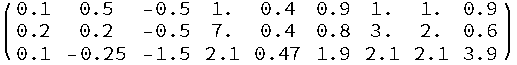
\includegraphics{refHmat.pdf}}}\intertext{with $\psi_c=\psi_\epsilon=0, \,\,  \psi_z=I$.
These coefficients are not completely arbitrary in so far as the series 
representation requires that the linear model
has a unique stable solution.\footnote{I have chosen $H_1$ full rank to span the space for the 3 arbitrary independent $z_t$ time series.}}
  B=
\vcenter{\hbox{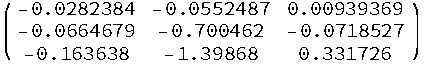
\includegraphics{refBmat.pdf}}}\\
\phi=
\vcenter{\hbox{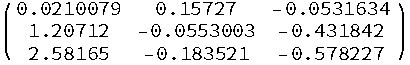
\includegraphics{refPhimat.pdf}}}\\
F=
\vcenter{\hbox{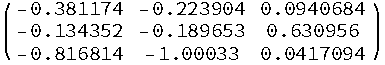
\includegraphics{refFmat.pdf}}}
\end{gather} 



The existence of a series 
representation requires only the spanning condition and the requirement that the state values along the 
paths remain bounded.  For example, consider the following three
bounded families of time series paths:
\begin{gather}
  x_{1,t}=\frac{\someNorm{x_{t-1}}}{{1+\someNorm{\epsilon_{t}}}} D_\pi(t) \intertext{where $D_\pi(t)$ gives the t-th digit of $\pi$}
x_{2,t}=\frac{\someNorm{x_{t-1}}}{({1+\someNorm{\epsilon_{t}}})^2} (-1)^t\\
x_{3,t}=\epsilon_t \intertext{and the $\epsilon_t$ are a sequence of pseudo random draws from the uniform distributions $\mathcal{U}(-4,4)$} \,\, \text{ produced subsequent to the selection of a random seed. $randomseed(\someNorm{x_{t-1}}+\someNorm{\epsilon_t})$}
\end{gather} 
The upper three panels in Figure \ref{arbpaths} display these three time series. The first set of trajectories characterizes 
a function of the digits in the decimal representation of $\pi$.  
The second set of trajectories  oscillates between two values
determined by  a nonlinear function of the initial conditions, $x_{t-1}$ and the shock.
The third set of trajectories characterizes a sequence of uniformly distributed random numbers based on a seed determined by  a nonlinear function of  the initial conditions and the shock.
These paths were chosen to emphasize that the trajectories
 need not converge to a fixed point, and 
need not be produced by some linear rational expectations solution or by the iteration of a discrete-time map.
The spanning condition and the boundedness of the paths are  sufficient conditions for the existence 
of the series representation based on the ``almost arbitrary'' linear reference model,$\linMod$.\footnote{Although potentially useful in some contexts,
this paper will not investigate representations for families of
unbounded trajectories.}


\begin{figure}
  \centering
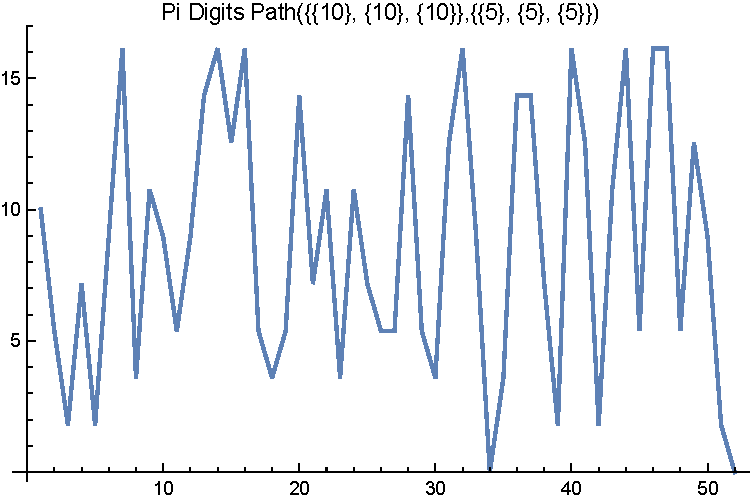
\includegraphics[width=2in]{piPath.pdf}
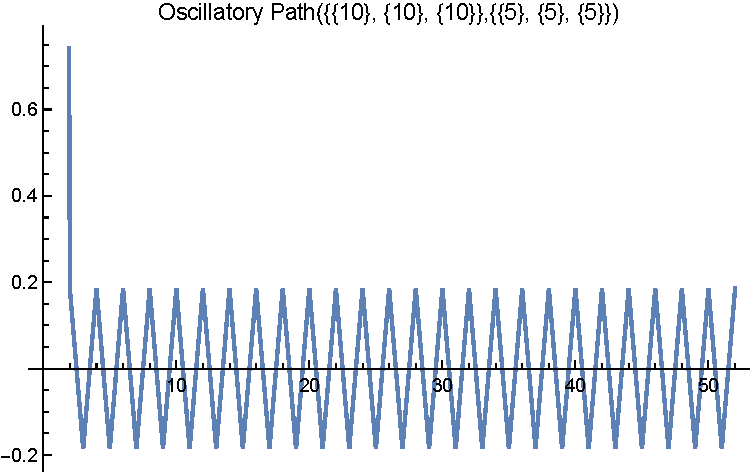
\includegraphics[width=2in]{oscillPath.pdf}
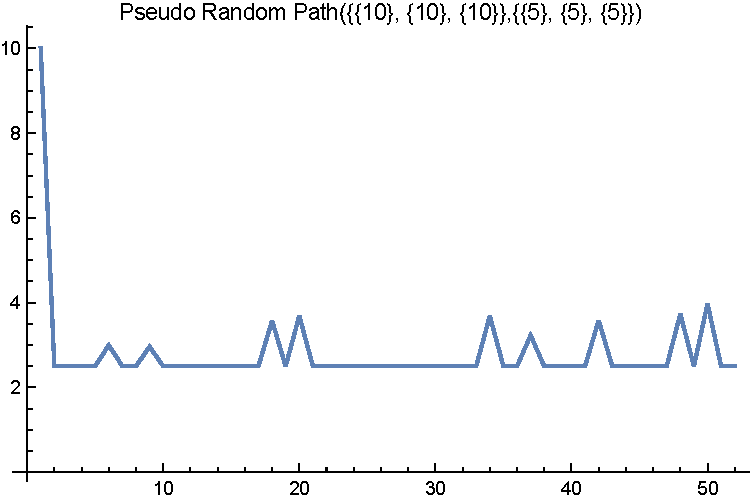
\includegraphics[width=2in]{pseudoPath.pdf}
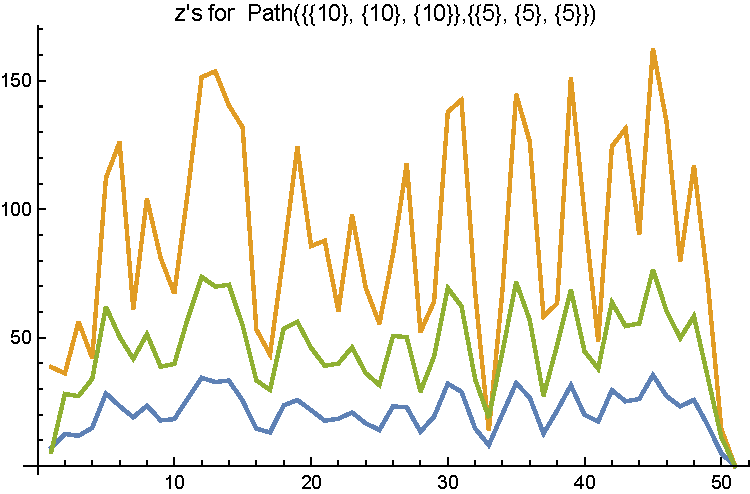
\includegraphics[width=3in]{theZs.pdf}  
  
  \caption{Arbitrary Bounded Time Series Paths and Corresponding $z_{i,t}$ values}\label{arbpaths}
\end{figure}





Figure \ref{arbpaths} also shows, for a particular initial state vector and shock value,  the paths for the   z's that generate the corresponding $x_t$ path.
One can repeat the calculations for any given initial condition to produce
a z series exactly replicating the new set of trajectories.  Thus, the family
of z functions along with equation \ref{theSeries} provide a series 
representation for the entire family of trajectories. Numerical linear algebra calculations can easily transform a $z_t$ series into an $x_t$ series and vice versa.





\subsection{Assessing $x_t$ Errors}
\label{sec:truncationerr}
The formula \ref{theSeries} was derived in \citep{anderson10}
to compute the impact on the current state of fully anticipated future shocks.  The formula characterizes the impact exactly.  However one can contemplate the impact of at least two deviations from the exact calculation:
\begin{enumerate}
\item One could truncate a series of correct values of $z_t$.  
\item One might have imprecise values of $z_t$ along the path.
\end{enumerate}
\subsubsection{Truncation Error}


The series representation can compute the entire series to machine precision
if all the terms are included, but, it will be useful to notice that
the terms for state vectors closer 
to the initial time have the most important impact.
One could consider approximating  $\mathcal{X}_t$ by 
truncating the series \ref{theSeries} at a finite number of terms.
 	 \begin{gather}
 	 \xWOargK_t \equiv B x_{t-1}+ \phi \psi_\epsilon\epsilon  + (I - F)^{-1} \phi \psi_c + \sum_{s=0}^k F^s \phi z_{t}\label{theTruncSeries}
 \end{gather}
We can bound the  series approximation truncation errors.
Since
    \begin{gather}
      \label{eq:1}
\sum_{s=k+1}^{\infty} F^s \phi \psi_z = (I -F)^{-1} F^{k+1}\phi \psi_z       \\
\infNorm{\xWarg-\xWargK} \le \infNorm{(I -F)^{-1} F^{k+1}\phi \psi_z} \left ( \infNorm{H_{-1} }+ \infNorm{H_{0} }+ \infNorm{H_{1} } \right )\bar{\mathcal{X}}
    \end{gather}
Again, note that for approximating $\xWarg$ the impact of  a given realization along the path declines for those realizations which are  more temporally distant.

 Figure \ref{figArbTrunc} shows
that this truncation error bound is a very conservative measure of the accuracy
of the truncated series.  The orange line represents the computed bound of
the infinity norm of the difference between $x_t$ from the full series and a truncated series for different lengths of the truncation.  The blue line shows the infinity norm of the actual difference between the $x_t$ computed using the full series and the value obtained using a truncated series.  The series requires only the first 20 terms to compute
the initial value of the state vector to machine precision. 


\begin{figure}
  \centering


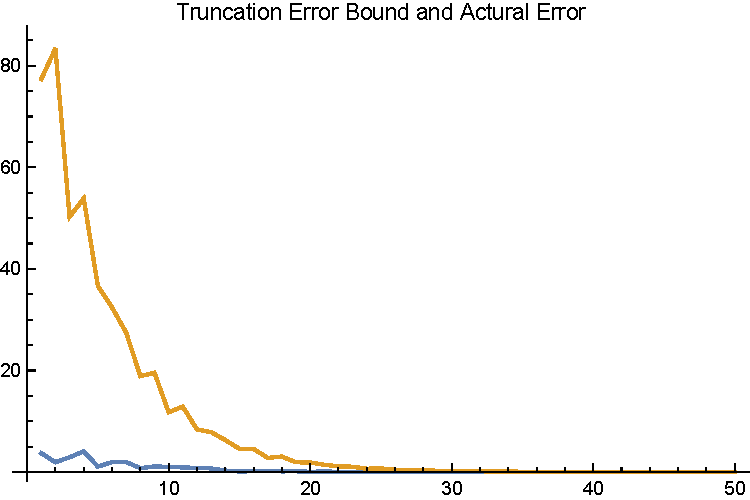
\includegraphics[width=3in]{arbTruncErr.pdf}  
  \caption{$x_t$ Error Bound Versus Actual Error} \label{figArbTrunc}

\end{figure}

\subsubsection{Path Error}


We can assess the impact of perturbed values for $z_t$ by computing the maximum discrepancy required for the $z_t$ and applying the 
partial sum formula
Thus, one can  approximate $\mathcal{X}_t$ using
 	 \begin{gather}
 	 \xWOargK_t \equiv B x_{t-1}+ \phi \psi_\epsilon\epsilon  + (I - F)^{-1} \phi \psi_c + \sum_{s=0}^\infty F^s \phi (z_{t}+\Delta z_{t})\label{theDeltaSeries}
 \end{gather}
Note yet again that for approximating $\xWarg$ the impact of  a given realization along the path declines for those realizations which are  more temporally distant.
However, we can conservatively bound the  series approximation  errors by using the largest $\Delta z_t$ in the formula:
    \begin{gather}
\infNorm{\xWarg-\xWargK} \le \infNorm{(I -F)^{-1} \phi \psi_z}  \infNorm{\Delta z_t } \label{pathErr}
    \end{gather}


\label{sec:pathnorm}

\section{Dynamic Stochastic Time Invariant Maps}
\label{sec:extToMaps}



\subsection{Application to Time Invariant Maps}



Many dynamic stochastic models have solutions that 
fall in the class of bounded time invariant maps.
As we have seen bounded time invariant maps can 
be represented using the framework from section \ref{sec:newseries}.

These time invariant maps impose additional structure on the time 
series they generate that allows us to use the series formula to
develop bounds for the error in the solution.
In this section, to keep things simple, we will begin with a familiar three equation system?\footnote{
Later, in order to handle models with regime switching and occasionally binding constraints, will need to consider more complicated collections of 
of equation systems with  Boolean gates. We will show how to apply the 
series formulation and to get error bounds for these models as well.}


\subsection{An RBC Example}
\label{sec:rbcaux}
  We consider a model described in \cite{Maliar2005}\footnote{Here, we set their $\beta=1$ do not discuss quasi-geometric discounting or time-inconsistency.}
 \begin{gather*}
   \max\left \{  u(c_t) + E_t \sum_{t=1}^\infty  \delta^{t}u(c_{t+1})\right \}\\
c_t + k_t=(1-d)k_{t-1} + \theta_t f(k_t)\\
f(k_t)= k_t^\alpha\\
u(c)=\frac{c^{1-\eta}-1}{1-\eta}
 \end{gather*}
The first order conditions for the model are

\begin{tcolorbox}[ams gather]
\frac{1}{c_t^{\eta}}=\alpha \delta k_{t}^{\alpha-1} E_t \left (\frac{\theta_{t+1}}{c_{t+1}^\eta} \right ) \\
c_t + k_t=\theta_{t-1}k_{t-1}^\alpha \\
 \theta_t =\theta_{t-1}^\rho e^{\epsilon_t}\label{rbcSys}
 \end{tcolorbox}
\label{sec:rbcexample}

It is well know that when $\eta=d=1$, we have a closed form solution\citep{lettau03}:
\begin{gather}
x_t(\xtmEpsArg)\equiv    \DR(\xtmEpsArg)\equiv
   \begin{bmatrix}
     c_t(\xtmEpsArg)\\k_t(\xtmEpsArg)\\ \theta_t(\xtmEpsArg)
   \end{bmatrix}=
   \begin{bmatrix}
(1-\alpha \delta) \theta_{t} k_{t-1}^\alpha\\
  \alpha \delta \theta_{t} k_{t-1}^\alpha.\label{soln}\\
\theta_{t-1}^\rho e^{\epsilon_t}.
   \end{bmatrix}
\end{gather}
For mean zero iid $\epsilon_t$ we can easily 
compute the conditional expectation of the model variables for any given $\theta_{t+k},k_{t+k}$
\begin{gather*}
  \DRCE(x_{t+k+1})\equiv
  \begin{bmatrix}
  E_t(c_{t+k+1}|\theta_{t+k},k_{t+k})\\
  E_t(k_{t+k+1}|\theta_{t+k},k_{t+k})\\
  E_t(\theta_{t+k+1}|\theta_{t+k},k_{t+k})
  \end{bmatrix}=
  \begin{bmatrix}
(1-\alpha\delta)k_{t+k}^\alpha e^{\frac{\sigma^2}{2}}\theta_{t+k}^\rho\\
\alpha\delta k_{t+k}^\alpha e^{\frac{\sigma^2}{2}}\theta_{t+k}^\rho\\
e^{\frac{\sigma^2}{2}}\theta_{t+k}^\rho
  \end{bmatrix}
\end{gather*}
Consequently, by applying the law of iterated expectations, we can compute conditional expected solution paths forward from any initial value $x_{t-1}$
and realization of $\epsilon_t$.
Subsequently, we can use the family of conditional expectations paths 
along with a contrived linear reference model to recover an 
approximation for equation \refeq{soln} along with error bounds.
Economists have long used similar manipulation of
time series paths for dynamic models. 
Indeed, Potter constructs his generalized impulse response functions using
differences in conditional expectations paths.\cite{Potter2000,Koop1996a}
Here, the series representation will provide a weighted sum of $z_t\tArg$ functions that give us an approximation for the known model solution.


For any given values of $k_{t-1},\theta_{t-1}, \epsilon_t$, the model solution and conditional expectations path:
\begin{gather*}
  \xWOarg_t(\xtmEpsArg)=\DR(\xtmEpsArg)\\
  \xWOarg_{t+k+1}(\xtmEpsArg)=\DRCE(\xWOarg_{t+k}(\xtmEpsArg))
\end{gather*}
produces paths for $\{(z_{1t}\tArg, z_{2t}\tArg, z_{3t}\tArg),\ldots\}$
\begin{gather*}
  z_{t+k} \equiv H_{-1} \xWOarg_{t+k-1} +  H_0 \xWOarg_{t+k} +  H_1 \xWOarg_{t+K+1} 
\end{gather*}
Formula \refeq{theSeries} requires that
\begin{gather*}
%   \begin{bmatrix}
% c_t(k_{t-1},\theta_{t-1}, \epsilon_t)\\
% k_t(k_{t-1},\theta_{t-1}, \epsilon_t)\\
% \theta_t(k_{t-1},\theta_{t-1}, \epsilon_t)
%   \end{bmatrix} \rightarrow
%   \begin{bmatrix}
%   z_{1t}(k_{t-1},\theta_{t-1}, \epsilon_t)\\
%   z_{2t}(k_{t-1},\theta_{t-1}, \epsilon_t)\\
%   z_{3t}(k_{t-1},\theta_{t-1}, \epsilon_t) 
%   \end{bmatrix}\equiv z(k_{t-1},\theta_{t-1}, \epsilon_t)\intertext{where}
%   \begin{bmatrix}
% c_t(k_{t-1},\theta_{t-1}, \epsilon_t)\\
% k_t(k_{t-1},\theta_{t-1}, \epsilon_t)\\
% \theta_t(k_{t-1},\theta_{t-1}, \epsilon_t)
%   \end{bmatrix}  =
\xWOarg(\xtmEpsArg)=
B   \begin{bmatrix}
c_{t-1}\\
k_{t-1}\\
\theta_{t-1}
  \end{bmatrix}  + \phi \psi_\epsilon\epsilon_t + (I - F)^{-1} \phi \psi_c + \sum_{\sForSum=0}^\infty F^s \phi z_{t+\sForSum}(k_{t-1},\theta_{t-1}, \epsilon_t) 
\end{gather*}
% \footnote{
% We need not  make these adjustments for the steady state,
% but doing so economizes on the number of terms 
% required for a given level of approximation
% accuracy.}

For example, using $d=1$ and the following parameter values and using the arbitrary linear reference model we can generate a series representation for the model solutions.

\begin{gather}\label{rbcparams}
\vcenter{\hbox{\includegraphics{../../paperProduction/occBind/docs/RBCParamSubs.pdf}}} \,\, \text{ we have } \,\,
  \begin{bmatrix}
    c_{ss}\\k_{ss} \\ \theta_{ss} 
  \end{bmatrix}=
\left [ \vcenter{\hbox{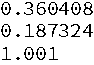
\includegraphics{RBCSSVal.pdf}}}\right ]
\end{gather}

With 
\begin{gather}\label{theInits}
  \begin{bmatrix}
 k_{t-1}\\\theta_{t-1}\\\epsilon_t 
  \end{bmatrix}=
\left [ \vcenter{\hbox{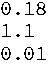
\includegraphics{anXEps.pdf}}}\right ]
\end{gather}


\begin{figure}
  \centering
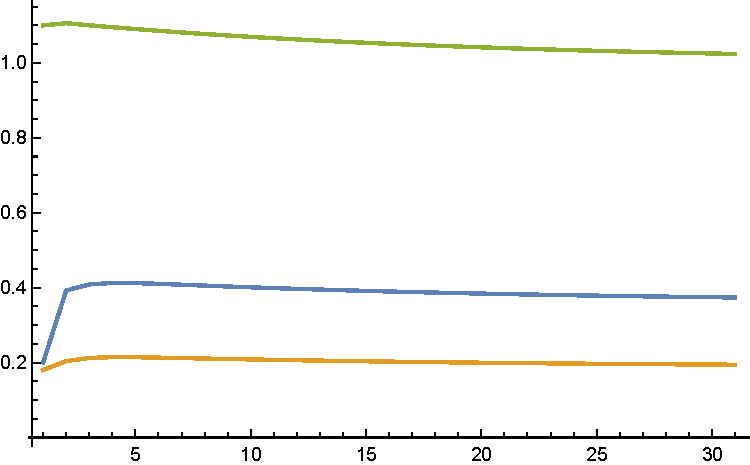
\includegraphics[width=2.5in]{simprbcvals.pdf}  \hspace{.75in}
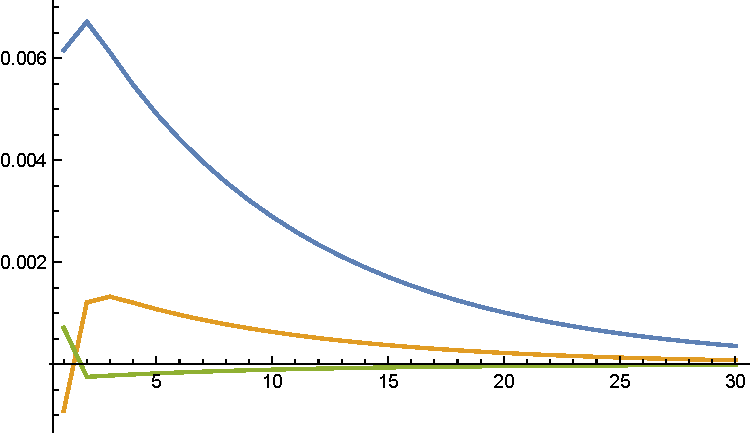
\includegraphics[width=2.5in]{simprbczvals.pdf}  
  \caption{model variable values and z values}
  \label{rbcpaths}
\end{figure}

The left panel of Figure \refeq{rbcpaths} shows the paths, from top to bottom, of $\theta_t, c_t, \text{ and } k_t$ from the initial values given in Equation \refeq{theInits}.  The right panel shows the paths for the $z_t$ variables associated with the linear reference model. The orange line corresponds to $z_{1t}\tArg$,
the blue line corresponds to $z_{2t}\tArg$ and the green line corresponds to $z_{3t}\tArg$.\footnote{For now we focus on the times series paths, $z_t(x_{t-1},\epsilon_t)$ for given $(x_{t-1},\epsilon_t)$.  Later we will exploit the information available from explicit investigation of the variation in
  $z_t(x_{t-1},\epsilon_t)$ with $(x_{t-1},\epsilon_t)$ to improve solution accuracy and robustness.}

Figure \ref{rbcTrunc} shows the impact that truncating the series has 
on the time t values of the state variables.   The bound for the error, $B_n$, shown in red 
 is again very pessimistic compared to the actual error, $Z_n$, shown in blue.
With enough terms, even using an ``almost'' arbitrarily chosen linear model,  the series approximation provides a machine precision accurate value for the time t state vector.  

\begin{figure}
  \centering
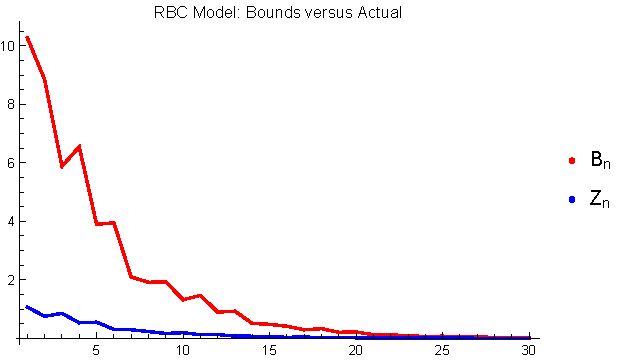
\includegraphics[width=2.7in]{simpArbBoundsVActual.pdf}  
  \caption{RBC Known Solution Truncation Error Bound Versus Actual: ``Almost Arbitrary'' Linear Reference Model}
  \label{rbcTrunc}
\end{figure}
\begin{figure}
  \centering
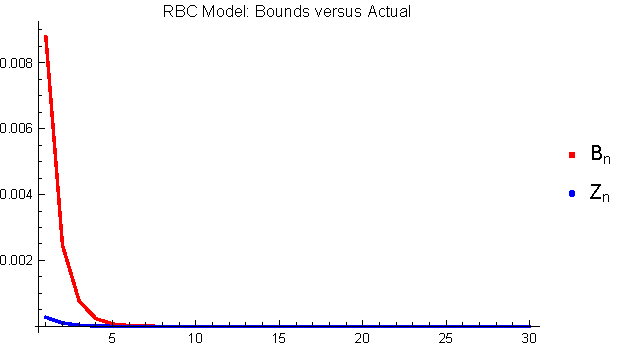
\includegraphics[width=2.7in]{simpBoundsVActual.pdf}  
  \caption{RBC Known Solution Truncation Error Bound Versus Actual: Stochastic Steady State Linearization Linear Reference Model}
  \label{rbcTruncSimp}
\end{figure}



Figure \ref{rbcTruncSimp} shows that using a 
linearization that better tracks the 
nonlinear model paths, improves the approximation $Z_n$, shown in blue  and the error bound $B_n$ shown in red.
Using the linearization of the RBC model produces a tighter but still pessimistic bound on the errors for the initial state vector.
Again, the first few terms make most of the difference in approximating the value of the state variables.


\subsection{A Convenient Model Specification Constraint}
\label{sec:convenient}



For convenience of notation in what follows, 
we will focus on models built up from components of the form
\begin{gather}
  h_i(x_{t-1},x_{t},x_{t+1},\epsilon_t)=h^{det}_{io}(x_{t-1},x_{t},\epsilon_t)+\sum_{j=1}^{p_i} [h^{det}_{ij}(x_{t-1},x_{t},\epsilon_t)h^{nondet}_{ij}(x_{t+1})]=0
\end{gather}
This is a very broad class of models including most widely used
macroeconomics models.

For example, the Euler equations for the  neoclassical growth  model 
\label{sec:simple-rbc-model-ext} can be written as
\begin{gather}
h_{10^{det}}(\cdot)=\frac{1}{c_t^\eta},\,\,
h_{11}^{det}()=\alpha \delta k_{t}^{\alpha-1} ,\,\,
h_{11}^{nondet}(\cdot)=E_t \left (\frac{\theta_{t+1}}{c_{t+1}^\eta} \right )\\
h_{20}^{det}(\cdot)=c_t + k_t-\theta_tk_{t-1}^\alpha,\,\,
h_{21}^{det}(\cdot)=0\\
h_{30}^{det}(\cdot)=\ln \theta_t -(\rho \ln \theta_{t-1} + \epsilon_t),\,\,
h_{31}^{det}(\cdot)=0
\end{gather}
Since we would otherwise  need to compute 
the conditional expectation of nonlinear expressions,  
this setup will make it possible for us to use auxiliary
variables to correctly compute the required expected values.

It is worth noting that since we will be working with models where expectations are computed at time t, with  $\epsilon_t$  known,  the only stochastic components are those with time subscripts greater than $t$. 





We can reconstruct our linear reference model by increasing its dimension by one  to accommodate 
 augmenting the RBC model with the equation
\begin{tcolorbox}[ams gather]
  \rcpC_t=\frac{\eta}{c_t}
\end{tcolorbox}
\noindent
substituting $\rcpC_{t+1}$ for $\frac{\eta}{c_{t+1}}$ in the first equation and 
 linearizing the RBC model about the ergodic mean
given in \refeq{rbcparams} leads to:
{\small
\begin{gather}
  \begin{bmatrix}
H_{-1}&H_{0}&H_{1} 
  \end{bmatrix}=\\
\vcenter{\hbox{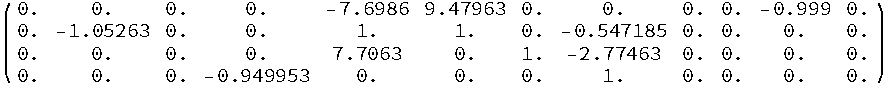
\includegraphics{RBCHmatSymb.pdf}}} \label{rbcLinSys}
\intertext{with}
\psi_\epsilon=
\begin{bmatrix}
  0\\0\\1\\0
\end{bmatrix}, \psi_z=I
\end{gather}%(\footnote{generated by AMAPaperCalcs.mth {RBCHmatSymb.pdf}})
}
Of course, these coefficients again produce a unique stable linear solution.

\begin{gather}
  B=
\vcenter{\hbox{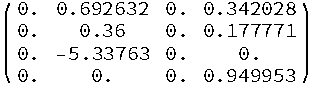
\includegraphics{RBCBmatSymb.pdf}}},
\phi=
\vcenter{\hbox{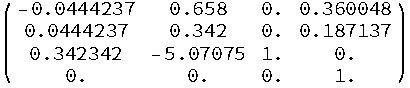
\includegraphics{RBCPhimatSymb.pdf}}}\\
F=
\vcenter{\hbox{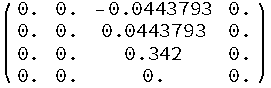
\includegraphics{RBCFmatSymb.pdf}}}\\
\psi_c=\vcenter{\hbox{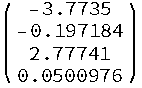
\includegraphics{RBCPsissSymb.pdf}}}
\end{gather}

Recomputing the truncation errors with the expanded model produces identical results for the original variables.


\section{Computing Model Solution Error Bounds}
\label{sec:solnerrorbounds}


The paper shows how to write a series representation for any proposed
model solution and to characterize the series representation for a typically
unknown solution in such a way that one can use the model equation errors  to construct an error bound for the norm of the distance between the proposed and the exact solution.

This work contrast with the analysis provided in
\cite{judd2017lower,peralta-alva14,santos2005accuracy,Santos2000accuracy}. 
Their approaches identify Euler Equation Errors, but use statistical techniques to estimate the impact of these errors on solution accuracy.  Here we compute
an equation for the bound that does not require statistical inference.





\subsection{The Error Bound Formula}
\label{sec:errorformula}


We consider time invariant maps such as often arise from solving an
 optimization problem codified in a systems of equations.  
In what follows, we construct an error bound for proposed model solutions.
Consider a bounded region, $\bndRgn$, where all iterated conditional expectations paths remain bounded.
 Given an exact solution $x^\star_t=g^\star(x_{t-1},\epsilon_t)$ define the conditional expectations function,
  \begin{gather}
G^\star(x)\equiv\expct{g^\star(x,\epsilon)} \intertext{then with}
E_tx^\star_{t+1}=G^\star(g^\star(x_{t-1},\epsilon_t)) \intertext{we have}
    \label{eq:2}
\eqnFunc(x^\star_{t-1},x^\star_t,E_tx^\star_{t+1},\epsilon_t)=0  \,\, \forall  (x_{t-1},\epsilon_t)\\ \intertext{In words, the exact solution  exactly satisfies the model equations.  Using $G^\star$ and $\linMod$, construct the family of trajectories and corresponding $z^\star_t(x_{t-1},\epsilon)$ }
   x^\star_t(x_{t-1},\epsilon_t) \in{R^L}\,\,\infNorm{x^\star_t(x_{t-1},\epsilon_t)}  \le \bar{\mathcal{X}}\,\,\forall t\ > 0
  \end{gather}
   \begin{align}
   z^\star_{t}(x_{t-1},\epsilon_t) \equiv& H_{-1}  x^\star_{t-1}(x_{t-1},\epsilon_t) + \nonumber\\
 & H_0  x^\star_{t}(x_{t-1},\epsilon_t) +   \\
 & H_1  x^\star_{t+1}(x_{t-1},\epsilon_t). \nonumber
   \end{align}




   Consequently, the exact solution has a representation given by
	 \begin{gather}
	 x^\star_{t}(x_{t-1},\epsilon) =B x_{t-1}+ \phi \psi_\epsilon\epsilon + (I - F)^{-1} \phi \psi_c +\\ \sum_{\sForSum=0}^\infty F^s \phi z^\star_{t+\sForSum}(x_{t-1},\epsilon) \intertext{and}
	 \expct{x^\star_{t+1}(x_{t-1},\epsilon)} =B x^\star_{t+k} + \sum_{\sForSum =0}^\infty F^\sForSum \phi \expct{z^\star_{t+1+\sForSum}(x_{t-1},\epsilon)} + (I - F)^{-1} \phi \psi_c 
 \intertext{with}
 \eqnFunc(x_{t-1},x^\star_t,E_tx^\star_{t+1},\epsilon_t)=0  \,\, \forall  (x_{t-1},\epsilon_t)\\ 
	 \end{gather}

Now consider a proposed solution for the model,
 $x^p_t=g^p(x_{t-1},\epsilon_t)$ define
$G^p(x)\equiv\expct{g^p(x,\epsilon)}$  so that 
  \begin{gather*}
E_tx_{t+1}=G^p(g^p(x_{t-1},\epsilon_t))\\
\mathbf{e}_t^p(x_{t-1},\epsilon)\equiv
\eqnFunc(x_{t-1},x^p_t,E_tx^p_{t+1},\epsilon_t)
\end{gather*}
By construction,  the conditional expectations paths will all be bounded
in the region $\bndRgn^p$. Using $G^p$ and $\linMod$ construct the family of trajectories and corresponding $z^p_t(x_{t-1},\epsilon)$\footnote{The algorithm presented below for finding solutions provides a mechanism for generating such proposed solutions.} 
\begin{gather*}
   x^p_t(x_{t-1},\epsilon_t) \in{R^L}\,\,\infNorm{x^p_t(x_{t-1},\epsilon_t)}  \le \bar{\mathcal{X}}\,\,\forall t\ > 0
  \end{gather*}
   \begin{align}
   z^p_{t}(x_{t-1},\epsilon_t) \equiv& H_{-1}  x^p_{t-1}(x_{t-1},\epsilon_t) + \nonumber\\
 & H_0  x^p_{t}(x_{t-1},\epsilon_t) +   \\
 & H_1  x^p_{t+1}(x_{t-1},\epsilon_t). \nonumber
   \end{align}








 The proposed solution has a representation given by 
  \begin{gather}
    \label{eq:4}
	 x^p_{t}(x_{t-1},\epsilon) =B x_{t-1}+ \phi \psi_\epsilon\epsilon + (I - F)^{-1} \phi \psi_c +\\ \sum_{\sForSum=0}^\infty F^s \phi z^p_{t+\sForSum}(x_{t-1},\epsilon) 
 \intertext{and}
 	 \expct{x^p_{t+1}(x_{t-1},\epsilon)} =B x^p_{t+k} + \sum_{\sForSum =0}^\infty F^\sForSum \phi z^p_{t+1+\sForSum}(x_{t-1},\epsilon) + (I - F)^{-1} \phi \psi_c \intertext{with}
\mathbf{e}_t^p(x_{t-1},\epsilon)\equiv
\eqnFunc(x_{t-1},x^p_t,E_tx^p_{t+1},\epsilon_t)
  \end{gather}




  \begin{gather}
    \label{eq:3}
	 x^\star_{t}(x_{t-1},\epsilon) -	 x^p_{t}(x_{t-1},\epsilon) =
         \sum_{\sForSum=0}^\infty F^s \phi (z^\star_{t+\sForSum}(x_{t-1},\epsilon)-z^p_{t+\sForSum}(x_{t-1},\epsilon))     \\
\Delta z_{t+\sForSum}^p(x_{t-1},\epsilon_t)         \equiv (z^\star_{t+\sForSum}(x_{t-1},\epsilon)-z^p_{t+\sForSum}(x_{t-1},\epsilon))\\
	 x^\star_{t}(x_{t-1},\epsilon) -	 x^p_{t}(x_{t-1},\epsilon) =
\sum_{\sForSum=0}^\infty F^s \phi \Delta z_{t+\sForSum}^p(x_{t-1},\epsilon_t)   \\ 
	\infNorm{ x^\star_{t}(x_{t-1},\epsilon) -	 x^p_{t}(x_{t-1},\epsilon)} \le
\sum_{\sForSum=0}^\infty F^s \phi \infNorm{\Delta z_{t+\sForSum}^p(x_{t-1},\epsilon_t)}    
  \end{gather}

  By bounding the largest deviation in the paths for the $\Delta z_t^p$ we can bound the largest difference in $x_t$.\footnote{Since the future values are probability weighted averages of the $\Delta z_t^p$ values for the given initial conditions and the condition expectations paths remain in the region $\bndRgn^p$,
the largest error for $\Delta z_{t+k}^p$   are pessimistic bounds for the errors from the conditional expectations path. } The exact solution satisfies the model equations exactly.  The error associated with the proposed solution leads to a conservative bound on the largest change in $z$ needed to match the exact solution.

  \begin{tcolorbox}[ams gather]
  \Delta z_t \le  
\max_{\{x_{-},\epsilon\}} \infNorm{ \phi \eqnFunc(x_{-},g^p(x_{-},\epsilon),G^p(g^p(x_{-},\epsilon)),\epsilon) }\\
	\infNorm{ x^\star_{t}(x_{t-1},\epsilon) -	 x^p_{t}(x_{t-1},\epsilon)} \le
\max_{\{x_{-},\epsilon\}} \infNorm{(I-F)^{-1} \phi \eqnFunc(x_{-},g^p(x_{-},\epsilon),G^p(g^p(x_{-},\epsilon)),\epsilon) }
  \end{tcolorbox}


\newcommand{\hApp}[1]{{H_-{#1}_{t-1} +H_0{#1}_t +H_+{#1}_{t+1}}}

  \begin{gather*}
z^\star_t=\hApp{x^\star}\\
z^p_t=\hApp{x^p}\\
0=\eqnFunc(x^\star_{t-1},x^\star_{t},x^\star_{t+1},\epsilon_t)\\
\mathbf{e}_t^p(x_{t-1},\epsilon)=\eqnFunc(x^p_{t-1},x^p_{t},x^p_{t+1},\epsilon_t)\\
\max \Delta z_t =\infNorm{H_0(x^p_t-x^\star_t)+H_+(x^p_{t+1}-x^\star_{t+1})}
\intertext{with}
\eqnFunc(x^p_{t-1},x^p_{t},x^p_{t+1},\epsilon_t) \le 
\mathbf{e}_t^p(x_{t-1},\epsilon)
  \end{gather*}

Use MSNTO to find constrained max.


\begin{verbatim}
Nelder–Mead

The Nelder–Mead method is a direct search method. For a function of variables, the algorithm maintains a set of points forming the vertices of a polytope in -dimensional space. This method is often termed the "simplex" method, which should not be confused with the well-known simplex method for linear programming.

At each iteration, points form a polytope. The points are ordered so that A new point is then generated to replace the worst point

Let be the centroid of the polytope consisting of the best points, . A trial point is generated by reflecting the worst point through the centroid, , where is a parameter.

If the new point is neither a new worst point nor a new best point, , replaces .

If the new point is better than the best point, , the reflection is very successful and can be carried out further to , where is a parameter to expand the polytope. If the expansion is successful, , replaces ; otherwise the expansion failed, and replaces .

If the new point is worse than the second worst point, , the polytope is assumed to be too large and needs to be contracted. A new trial point is defined as

where is a parameter. If , the contraction is successful, and replaces . Otherwise a further contraction is carried out.

The process is assumed to have converged if the difference between the best function values in the new and old polytope, as well as the distance between the new best point and the old best point, are less than the tolerances provided by AccuracyGoal and PrecisionGoal.

Strictly speaking, Nelder–Mead is not a true global optimization algorithm; however, in practice it tends to work reasonably well for problems that do not have many local minima.
\end{verbatim}


\subsection{Generalization and Practical Considerations for Applying the Formula}
\label{sec:practicalformula}

The framework provides a new way to bound the error one can expect from
employing a given proposed model solution and leads, in Section \ref{sec:algoforsoln},, to an
algorithm with  components similar to parameterized expectations that
one can use to improve proposed solutions. In that section, the
series representation makes
it possible to organize the calculation around computing a deterministic
problem at time t given a proposed solution.  The deterministic solution
can accommodate inequality constraints or alternative regimes to produce a
solution for each set of initial conditions.  One can typically arrange,
perhaps by adding auxiliary variables, to produce a ``decision rule''
that one can use to correctly precompute a deterministic conditional
expectation function that can be iterated forward and serves to
improve upon the original proposed solution.
Time invariant stochastic functions 
lead naturally to an associated family of deterministic maps
which can be conveniently represented by the series representation.


The paper studies a very general class of models whose 
solutions are characterized by $\eqnFuncSys$, a 
 exhaustive and mutually exclusive set of
of   model equations, $\eqnFunc_i$,  and Boolean valued gates, $\preGate_i$, $\postGate_i$. 
that together determine the solution  $x_t\tArg$
%\begin{gather}
%\intertext{ where, each }
%\eqnFuncSysI{i}\equiv \eqnFuncSysIExpl{i} \label{eqnGates}
%\end{gather}




To fix notation,  assume that we have a countable collection of equations systems that are mutually exclusive and exhaustive.
Given $(x_{t-1},\epsilon_t$,  this collection of 
systems of equations produces a unique solution for $x_t$.  We will include 
enough auxiliary variables so that we can correctly compute expected values
for model variables by applying the law of iterated 
expectations to individual variables.
To simplify the algorithm specification and implementation, assume that the
$x_t$ satisfies one and only one of the 
collection of equations and $x_t$ is (locally) the unique solution 
for the collection of
equations.  Examples of such systems include typical DSGE models that have one
system of equations, occasionally binding constraints with solutions demonstrating complementary slackness, regime switching models with systems corresponding to the status in each given regime or combinations of the above.  See the appendix for an example of a specification for occasionally binding constraints(\ref{sec:occbind}) and for regime switching)(\ref{sec:ressw}).

It will be convenient for describing the algorithms to
 augment the model equations to include auxiliary variables so that we can write the model in the form

\begin{gather}
\eqnFuncSys \intertext{ where, each }
\eqnFuncSysI{i}\equiv \eqnFuncSysIExpl{i} \label{eqnGates}
\end{gather}
 represents a set of model equations, $\eqnFunc_i$,  with a Boolean valued gate, $\preGate_i, \postGate_i$. Consequently, will will have an equation system and a gatekeeper logical expression indicating which equation system is in force for a given solution for a give $x_{t-1}, \epsilon_t$  They represent exhaustive and mutually exclusive equation systems determining the solution at time t for the model.  They could be complementary slackness conditions or could represent a model with different regimes. We will consider time invariant model solutions $x_t=\xWarg$.  Given $\xWarg$, $\XWOarg(x_{t-1})\equiv \expct{\xWarg}$. 





\section{Improving Proposed  Solutions}
\label{sec:algoforsoln}

\subsection{An Informal Characterization  of the Algorithm}
\label{sec:walkthrough}


Before presenting the pseudocode for the detailed algorithm, this section
describes  how the proposed approach differs from 
what is typically done for solving dynamic stochastic models.
In what follows, both the traditional and the new  approach use anisotropic
Smolyak polynomial function approximation with precomputed expectations.
This section uses the series representation to
compute the solution for the case when the exact solution is known and
to compare the various approximations to the known actual solution.

As with the standard approach it is important to iterate on the proposed solution until consistency between
the decision rule used for setting time t values and the expectations function for setting
$\expct{x_{t+1}}$ in the model equations.  Thirty iteration are more than enough for the standard and the new approach.
The new approach entails adding constraints on the time t state variables that
come from the series representation for the proposed solution.  The series
expression relates the time t values to the values along the anticipated
conditional expectations path.



\subsubsection{Approximating the Known Solution: $U(c) = Log(c)$ }
\label{sec:recov-known-solut}

Figure \ref{fig:erg}  characterizes the use of the parallelotope
transformation described in \cite{Judd2013}. The left panel shows the 200 values of $k_t$ and $\theta_t$ resulting from a stochastic simulation of the the known decision rule. The right panel shows the transformed variables that constitute
an improved set of variables for constructing function approximation values.
\begin{figure}
  \centering
  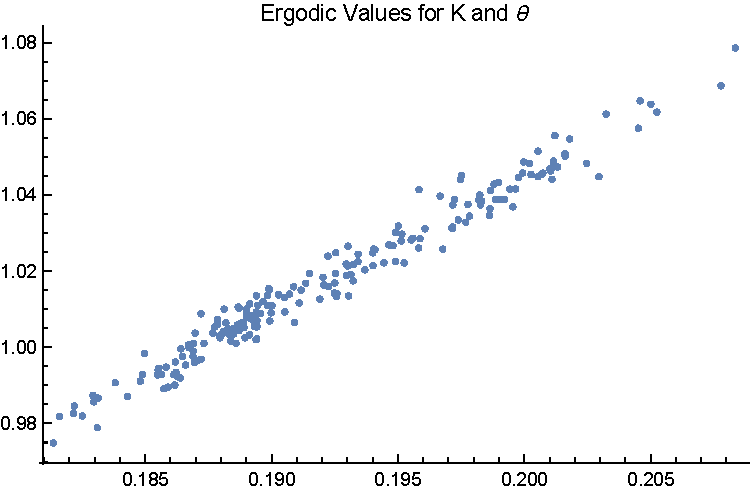
\includegraphics[width=2.5in]{ergodicKTheta.pdf}
  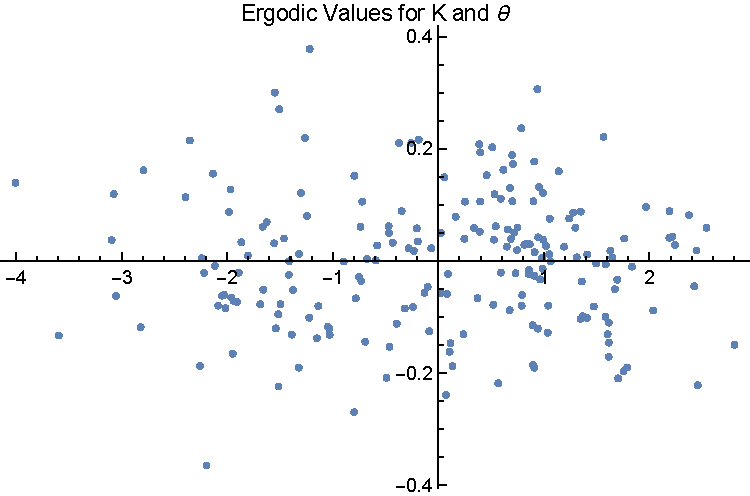
\includegraphics[width=2.5in]{ergodicZs.pdf}
  \caption{The Ergodic Values for $k_t, \theta_t$ }
  \label{fig:erg}
\end{figure}


\begin{gather}
\bar{X}= \vcenter{\hbox{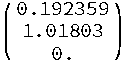
\includegraphics{ergodicMean.pdf}}}
\end{gather}
\begin{gather}
\sigma_{X}= \vcenter{\hbox{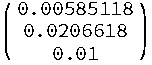
\includegraphics{ergodicSD.pdf}}}
\end{gather}


\begin{gather}
V= \vcenter{\hbox{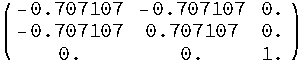
\includegraphics{ergodicV.pdf}}}
\end{gather}

\begin{gather}
\max U= \vcenter{\hbox{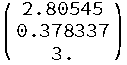
\includegraphics{ergodicMaxZ.pdf}}}
\end{gather}
\begin{gather}
\min U= \vcenter{\hbox{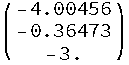
\includegraphics{ergodicMinZ.pdf}}}
\end{gather}


The following graphs present key characteristics of the solutions.  
The panels labeled approximation error show contour plots of $\mathbb{E}(z_{1,t-1},z_{2,t-1})$:
\begin{gather*}
\mathbb{E}(z_{1,t-1},z_{2,t-1})\equiv \sqrt{(c_t()-c_t^\star())^2 +(k_t()-k_t^\star())^2 +(\theta_t()-\theta_t^\star())^2 +(N_t()-N_t^\star())^2 }  
\end{gather*}
The panels labeled equation error show  contour plots for
\begin{gather*}
  \mathbb{D}(z_{1,t-1},z_{2,t-1})\equiv \eqnFunc(x_{-},g^p(x_{-},\epsilon),G^p(g^p(x_{-},\epsilon)),\epsilon). These are the model equation ``Euler'' errors.
\end{gather*}
The values of $U_t$ range over the ergodic set described above.

The bottom panel of
Figure \ref{fig:tradOne} shows the approximation error obtained by the standard
practice of selecting a number of approximation points and solving the collocation problem for the model equations at these points to
 approximate the  decision rule. The green dot shows the values of $(u_1,u_2)$ associated with the largest actual error.  The orange dot shows $(u_1,u_2)$ associated with  the largest equation system discrepancy 
and was used in computing the error bound. The black dots show the interpolation points. The label of the figure provides the predicted error bound along with the largest error.
The top panel provides a contour plot of the
norm of the equation errors. The bottom plot shows the error in the decision rule for different values of $k_{t-1}, \theta_{t-1}$ with $\epsilon_t=0$.
Notice that  setting $K=0$ is not equivalent to the standard approach as
the series formula has a correction term for $z_t(x_{t-1},\epsilon_t)$




\begin{figure}
  \centering
\ifmacosx


  \includegraphics{resDir/forBetterRBC--1,1,1-Iters30theK0host-MacBook-Pro-2numKern2ApproxTrad.pdf}

  \includegraphics{resDir/forBetterRBC--1,1,1-Iters30theK0host-MacBook-Pro-2numKern2Trad.pdf}

\fi
\iflinux
\includegraphics{resDir/forBetterRBC--1,1,1-Iters30theK0host-node015dnumKern16ApproxTrad.pdf}
\includegraphics{resDir/forBetterRBC--1,1,1-Iters30theK0host-node015dnumKern16ExactTrad.pdf}
\fi
  \caption{Contour Plot for traditional approx=(1,1,1) (Standard Approach)}
  \label{fig:tradOne}
\end{figure}


\begin{figure}
  \centering
\ifmacosx
  \includegraphics{resDir/forBetterRBC--1,1,1-Iters30theK0host-MacBook-Pro-2numKern2Approx.pdf}
  \includegraphics{resDir/forBetterRBC--1,1,1-Iters30theK0host-MacBook-Pro-2numKern2.pdf}
\fi
\iflinux
\includegraphics{resDir/forBetterRBC--1,1,1-Iters30theK0host-node015dnumKern16Approx.pdf}
\includegraphics{resDir/forBetterRBC--1,1,1-Iters30theK0host-node015dnumKern16.pdf}
\fi
  \caption{Contour Plot for approx=(1,1,1) K =0 }
  \label{fig:cntpltA}
\end{figure}




\begin{figure}
  \centering
\iflinux
\includegraphics[width=1.0in]{resDir/forBetterRBC--1,1,1-Iters30theK1host-node015dnumKern16.pdf}
\includegraphics[width=1.0in]{resDir/forBetterRBC--1,1,1-Iters30theK2host-node015dnumKern16.pdf}
\includegraphics[width=1.0in]{resDir/forBetterRBC--1,1,1-Iters30theK3host-node015dnumKern16.pdf}
\includegraphics[width=1.0in]{resDir/forBetterRBC--1,1,1-Iters30theK4host-node015dnumKern16.pdf}
\includegraphics[width=1.0in]{resDir/forBetterRBC--1,1,1-Iters30theK5host-node015dnumKern16.pdf}
\fi
\ifmacosx
\includegraphics[width=1.0in]{resDir/forBetterRBC--1,1,1-Iters30theK1host-MacBook-Pro-2numKern2.pdf}
\includegraphics[width=1.0in]{resDir/forBetterRBC--1,1,1-Iters30theK2host-MacBook-Pro-2numKern2.pdf}
\includegraphics[width=1.0in]{resDir/forBetterRBC--1,1,1-Iters30theK3host-MacBook-Pro-2numKern2.pdf}
\includegraphics[width=1.0in]{resDir/forBetterRBC--1,1,1-Iters30theK4host-MacBook-Pro-2numKern2.pdf}
\includegraphics[width=1.0in]{resDir/forBetterRBC--1,1,1-Iters30theK5host-MacBook-Pro-2numKern2.pdf}
\fi
\iflinux
\includegraphics[width=1.0in]{resDir/forBetterRBC--1,1,1-Iters30theK1host-node015dnumKern16.pdf}
\includegraphics[width=1.0in]{resDir/forBetterRBC--1,1,1-Iters30theK2host-node015dnumKern16.pdf}
\includegraphics[width=1.0in]{resDir/forBetterRBC--1,1,1-Iters30theK3host-node015dnumKern16.pdf}
\includegraphics[width=1.0in]{resDir/forBetterRBC--1,1,1-Iters30theK4host-node015dnumKern16.pdf}
\includegraphics[width=1.0in]{resDir/forBetterRBC--1,1,1-Iters30theK5host-node015dnumKern16.pdf}
\fi
  \caption{Contour Plot for approx=(1,1,1)  K =1,2,3,4,5}
  \label{fig:cntpltB}
\end{figure}



The panels in Figure \ref{fig:cntpltB} shows the results when $K=1,2,3,4,5$
while 
Figure \ref{fig:cntpltC} shows the results when $K=10$, with degree of approximation $(1,1,1)$
for computing the decision rule.  The top panel provides a contour plot of the
norm of the equation errors. The bottom plot shows the error in the decision rule for different values of $k_{t-1}, \theta_{t-1}$ with $\epsilon_t=0$.  The plots for different values of $\epsilon_t$ are not different.  The error bound, 
\ifmacosx
\input{resDir/forBetterRBC--1,1,1-Iters30theK30host-MacBook-Pro-2numKern2errBnd.tex} 
\fi
is 25\% larger than the actual error 
\iflinux
%\input{resDir/forBetterRBC--1,1,1-Iters30theK30host-MacBook-Pro-2numKern111acterr.tex} 
\fi
%  Notice that even though equation errors are comparable in magnitude, the error in the decision rule is significantly smaller for the series representation solution.  The additional constraints on the equation system provided by computing conditional expectations paths and incorporating them into the solution at time $t$ leads to better solutions.



% In what follows I show the impact of increasing the number of terms 
% employed in the series representation.  



Figure \ref{fig:cntpltA} shows the results when $K=0$, with degree of approximation $(1,1,1)$.  The top panel provides a contour plot of the
norm of the equation errors. The bottom plot shows the error in the decision rule for different values of $k_{t-1}, \theta_{t-1}$ with $\epsilon_t=0$.  The plots for different values of $\epsilon_t$ are not appreciably different. The error bound, 
\ifmacosx
\input{resDir/forBetterRBC--1,1,1-Iters30theK0host-MacBook-Pro-2numKern2errBnd.tex} 
\fi
\iflinux
\input{resDir/forBetterRBC--1,1,1-Iters20theK0numKern0errBnd.tex} 
\fi
is 25\% larger than the actual error 
\ifmacosx
\input{resDir/forBetterRBC--1,1,1-Iters30theK0host-MacBook-Pro-2numKern2acterr.tex}
\fi
\iflinux
\input{resDir/forBetterRBC--1,1,1-Iters20theK0numKern16acterr.tex}
\fi



\begin{figure}
  \centering
\ifmacosx
  \includegraphics{resDir/forBetterRBC--1,1,1-Iters30theK30host-MacBook-Pro-2numKern2Approx.pdf}
  \includegraphics{resDir/forBetterRBC--1,1,1-Iters30theK30host-MacBook-Pro-2numKern2.pdf}
\fi
\iflinux
  \includegraphics{resDir/forBetterRBC--1,1,1-Iters30theK10host-node015dnumKern16Approx.pdf}
  \includegraphics{resDir/forBetterRBC--1,1,1-Iters30theK10host-node015dnumKern16.pdf}
\fi
  \caption{Contour Plot for approx=(1,1,1) iters 20 K =10}
  \label{fig:cntpltC}
\end{figure}


\begin{figure}
  \centering
\ifmacosx
  \includegraphics{resDir/forBetterRBC--1,1,1-Iters30theK30host-MacBook-Pro-2numKern2Approx.pdf}
  \includegraphics{resDir/forBetterRBC--1,1,1-Iters30theK30host-MacBook-Pro-2numKern2.pdf}
\fi
\iflinux
  \includegraphics{resDir/forBetterRBC--1,1,1-Iters30theK20host-node015dnumKern16Approx.pdf}
  \includegraphics{resDir/forBetterRBC--1,1,1-Iters30theK20host-node015dnumKern16.pdf}
\fi
  \caption{Contour Plot for approx=(1,1,1) iters 20 K =20}
  \label{fig:cntpltC}
\end{figure}


\begin{figure}
  \centering
\ifmacosx
  \includegraphics{resDir/forBetterRBC--1,1,1-Iters30theK30host-MacBook-Pro-2numKern2Approx.pdf}
  \includegraphics{resDir/forBetterRBC--1,1,1-Iters30theK30host-MacBook-Pro-2numKern2.pdf}
\fi
\iflinux
  \includegraphics{resDir/forBetterRBC--1,1,1-Iters30theK50host-node015dnumKern16Approx.pdf}
  \includegraphics{resDir/forBetterRBC--1,1,1-Iters30theK50host-node015dnumKern16.pdf}
\fi
  \caption{Contour Plot for approx=(1,1,1) iters 20 K =50}
  \label{fig:cntpltC}
\end{figure}

% \begin{figure}
%   \centering
% \iflinux  
% \includegraphics{resDir/forBetterRBC--2,2,2-Iters20theK0numKern5.pdf}
% \fi
% \ifmacosx  
% \includegraphics{resDir/forBetterRBC--2,2,2-Iters20theK0numKern2.pdf}
% \fi
%   \caption{Contour Plot for approx=(2,2,2) 20 iterations and K =0}
%   \label{fig:cntpltD}
% \end{figure}

% \begin{figure}
%   \centering
% \iflinux
%   \includegraphics{resDir/forBetterRBC--2,2,2-Iters20theK5numKern5.pdf}
% \fi
% \ifmacosx  
% \includegraphics{resDir/forBetterRBC--2,2,2-Iters20theK5numKern2.pdf}
% \fi
%   \caption{Contour Plot for approx=(2,2,2) 20 iterations and K =5}
%   \label{fig:cntpltE}
% \end{figure}

% \begin{figure}
%   \centering
% \ifmacosx
%   \includegraphics{resDir/forBetterRBC--2,2,2-Iters20theK10numKern2.pdf}
% \fi
%   \caption{Contour Plot for approx=(2,2,2) 20 iterations and K =10}
%   \label{fig:cntpltF}
% \end{figure}

% \begin{figure}
%   \centering
% \ifmacosx
%   \includegraphics{resDir/forBetterRBC--2,2,2-Iters30theK30host-MacBook-Pro-2numKern2ApproxTrad.pdf}


%   \includegraphics{resDir/forBetterRBC--2,2,2-Iters30theK30host-MacBook-Pro-2numKern2.pdf}
% \fi
%   \caption{Contour Plot for approx=(2,2,2) 20 iterations and K =20}
%   \label{fig:cntpltG}
% \end{figure}
% \begin{figure}
%   \centering
% \ifmacosx
%   \includegraphics{resDir/forBetterRBC--2,2,2-Iters30theK30host-MacBook-Pro-2numKern2ApproxTrad.pdf}


%   \includegraphics{resDir/forBetterRBC--2,2,2-Iters30theK30host-MacBook-Pro-2numKern2.pdf}
% \fi
%   \caption{Contour Plot for approx=(2,2,2) 20 iterations and K =20}
%   \label{fig:cntpltH}
% \end{figure}
% \begin{figure}
%   \centering
% \ifmacosx
%   \includegraphics{resDir/forBetterRBC--2,2,2-Iters30theK30host-MacBook-Pro-2numKern2ApproxTrad.pdf}


%   \includegraphics{resDir/forBetterRBC--2,2,2-Iters30theK30host-MacBook-Pro-2numKern2.pdf}
% \fi
%   \caption{Contour Plot for approx=(2,2,2) 20 iterations and K =20}
%   \label{fig:cntpltJ}
% \end{figure}

% \begin{figure}
%   \centering
% \ifmacosx
%   \includegraphics{resDir/forBetterRBC--3,3,3-Iters20theK0numKern2.pdf}
% \fi
%   \caption{Contour Plot for approx=(3,3,3) 20 iterations and K =0}
%   \label{fig:cntpltH}
% \end{figure}

% \begin{figure}
%   \centering
% \ifmacosx
%   \includegraphics{resDir/forBetterRBC--3,3,3-Iters20theK10numKern2.pdf}
%   \fi
%   \caption{Contour Plot for approx=(3,3,3) 20 iterations and K =10}
%   \label{fig:cntpltI}
% \end{figure}


\begin{figure}
  \centering
\ifmacosx
  \includegraphics{resDir/forBetterRBC--3,3,3-Iters20theK20numKern2.pdf}
  \fi
\iflinux
  \includegraphics{resDir/forBetterRBC--3,3,3-Iters30theK0host-node015dnumKern16ApproxTrad.pdf}
  \includegraphics{resDir/forBetterRBC--3,3,3-Iters30theK0host-node015dnumKern16Trad.pdf}
\fi
  \caption{Contour Plot for approx=(3,3,3) 30 iterations Traditional}
  \label{fig:cntpltI}
\end{figure}

\begin{figure}
  \centering
\ifmacosx
  \includegraphics{resDir/forBetterRBC--3,3,3-Iters20theK20numKern2.pdf}
  \fi
\iflinux
  \includegraphics{resDir/forBetterRBC--3,3,3-Iters30theK20host-node015dnumKern16Approx.pdf}
  \includegraphics{resDir/forBetterRBC--3,3,3-Iters30theK20host-node015dnumKern16.pdf}
\fi
  \caption{Contour Plot for approx=(3,3,3) 20 iterations and K =20}
  \label{fig:cntpltI}
\end{figure}




% \begin{itemize}
% \item show describe $z_t(x_{t-1},\epsilon_t)$ for RBC
% \item start linear.  check error bounds, if adequate done
% \item traditional iteration ignores the path constraints on initial solution leading to larger errors on $\bndRgn^p$
% \item It's a good idea to compute easy approximation using just the linear model one ieration to get an approximation for the ergodic set
% \item PEA moving bounds \cite{maliarmovingbounds}
% \item them simulate and make the Maliar SVD transformation
% \item then iterate on the ergodic set till it settles down
% \item in this way can avoid solutions which are explosive when iterated 
% \item need to see if this works when honoring complimentary slackness
% \item not related to z transform. probably should change z's
% \end{itemize}

\subsection{Ergodic Partition of Invariant Sets}
\label{sec:ergod-part-invar}

Following \citep{ergodicvisual}, consider a map $T$ on a compact metric space $\mathcal{A}$ endowed with a measure $\mu$ preserved under $T$. We wish to 
visualize invariant sets $\mathcal{B} \subseteq \mathcal{A}$.

\begin{gather*}
  x_{t+1} =T x_t,\in A\,\,\forall t \in Z
\end{gather*}

\begin{gather*}
  x_0 \in B \implies T^t x_0 \in B \,\,\forall t \in Z
\end{gather*}

For ergodic invariant sets, consider $L^1$ real valued functions on A
\begin{gather*}
 f:A \rightarrow \mathbb{R}\in L^1(A) \iff \int_A |f(x)|dx <\infty
\end{gather*}

Define time average $f^\ast(x_0)$ of a function $f\in L^1(A)$ corresponding to a phase point $x_0\in A$
\begin{gather*}
  f^\ast(x_0)\equiv \lim_{t\rightarrow\infty} \frac{1}{t}\sum_{k=0}^{t-1}f(T^kx_0)
\end{gather*}

By the Ergodic Theorem, this limit exists almost everywhere ( a. e. ).
Call map T ergodic over $B \subset A$ if for a. . point  $x_0 \in B$ time average equals the space average for every function $f \in L^1(B)$ so that there exists an
ergodic measure.
\begin{gather*}
f^\ast(x_0) =\frac{1}{\mu_B(B)}\int_B f d\mu_B  
\end{gather*}
a.e. $B \subset A$

This implies $f^\ast$ is a constant a. e. in $B \subset A$  almost every orbit starting in B covers B densey at the limit.  Each $f^\ast$ is an invariant function $f^\ast(x_0)= f^\ast(T^tx_0) \, \forall t$  
The set of real numbers induces a partition of A called $\zeta_f\equiv \{B_a\}_{a\in\mathbb{R}}$ through a function $f\in L^1(A)$

\begin{gather*}
  B_a=(f^\ast)^{-1}(a), \,\,\forall a \in \mathbb{R}
\end{gather*}
Some of $B_a$ may be empty.

\begin{gather*}
  \mu\left (\bigcup_aB_a \right )=\mu(A),B_a\cap B_{a^\prime} = \emptyset ,\,\,\forall a \ne a^\prime
\end{gather*}
Denote set of points with no time average of $f$ by $\Sigma(f,T)$

\begin{gather*}
  A=(\cup_aB_a)\bigcup \Sigma(f,T)
\end{gather*}
To guarantee we don't lump what should be independent invariant sets together just because averages match, define using a collection of functions.
Final ergodic partation $\zeta_e$ product of all $zeta_f$ belonging to $S \subset L^1(A)$  Chose S as a basis for $L^1(A)$

\begin{gather*}
  \zeta_e= \bigvee_{f\in S} \zeta_f
\end{gather*}

Ergodic partition divides phase space into non-decomposable invariant sewts.  Can visualize using approximate ergodic partitions.

\begin{enumerate}
\item Set up a grid of initial grid-points
\item Pick N function $\{f_1,\ldots,f_N\}$ from $L^1(A)$ and compute partial time averages for $t_{final}$ iterations for each grid point.  These serve as approximations for $\{f_1^\ast,\ldots,f_N^\ast\}$
\item To every initial grid point associate the corresponding time average vector
  \begin{gather*}
    x \rightarrow \bar{f}(x),\,\, \bar{f}(x)\equiv \{f_1^\ast(x),\ldots,f_N^\ast(x)\}\in \mathbb{R}^N
  \end{gather*}
\item Observe the distribution of ime average vectors $\bar{f}$ and group them into clusters
\end{enumerate}


\subsection{Algorithm Overview}

% \subsubsection{Approximating an Unknown Solution: $U(c) \ne Log(c)$ }
 \label{sec:unknown-solutions}
The algorithm we have described,
uses a proposed deterministic map
characterizing the evolution of expected values for
the dynamic system going forward. It then solves
a deterministic problem at time t to improve the proposed solution.
There is nothing in the algorithm that precludes accommodating  inequality
constraints.\footnote{See section \ref{sec:regime-switch-model} characterizing
  models with regime switching.}


{
  \begin{itemize}
  \item Consider the single model case $  \eqnFunc(x_{t-1},x_t,\expct{x_{t+1}},\epsilon)=0$.  
\item We seek $\eqnFunc(x_{t-1},\xWOarg^\star\tArg,\XWOarg^\star(\xWOarg^\star\tArg),\epsilon)=0\,\,\forall \tArg $
\item Given a proposed model solution $x_t=\xWOarg^p\tArg$ compute $\XWOarg^p(x_{t-1})\equiv \expct{\xWOarg^p\tArg}$. 
\item we will use a linear reference model $\linMod  \equiv \linModMats$ 
to construct a series of $\zpWOarg$ functions that improve the accuracy of the proposed solution.
\end{itemize}
}



\begin{gather*}
 \intertext{We can define functions $\zpWOarg,\ZpWOarg$ by}
\zpWarg\equiv H
\begin{bmatrix}
x_{t-1}\\ \xpWarg\\ \XpWOarg(\xWarg)
\end{bmatrix}+\phi_\epsilon \epsilon_t+\phi_c\\
\ZpWOarg(x_{t-1})\equiv \expct{\zpWarg}
\end{gather*}
 \begin{itemize}
\item  {\color{blue}Algorithm loop begins here.} Define conditional expectations paths for $x_t, z_t$ 
 \begin{gather*}
 x_{t+k+1}=\XWOarg(x_{t+k}),\,\,\,z_{t+k+1}=\ZWOarg(x_{t+k})\,\,\,\,  \forall k\ge 0      \end{gather*}
% \item
% it will be useful to construct an augmented decision rule,
% $\ADR\tArg\equiv
%   \begin{bmatrix}
%     x^p\tArg\\z^p\tArg
%   \end{bmatrix}$, initially $z^p\tArg=0$
   \end{itemize}

{Using the $\zpWarg$ Series}
{\small
  \begin{itemize}
  \item We get expressions for $x_t,\,\, \expct x_{t+1}$ consistent with $\linMod$ and the conditional expectations path
   \begin{gather*}
     \mathcal{X}_{t} =B x_{t-1}+ \phi \psi_\epsilon\epsilon + (I - F)^{-1} \phi \psi_c + \sum_{\sForSum=0}^\infty F^s \phi \ZWOarg(x_{t+\nu})\\
	\expct{ \mathcal{X}_{t+1}} =B \mathcal{X}_{t}  + (I - F)^{-1} \phi \psi_c+ \sum_{\sForSum =0}^\infty F^{\sForSum-1} \phi \ZWOarg(x_{t+\nu}) \,\,\,\,\,\forall t,k \ge  0
\end{gather*}
\item Use the model equations, $\eqnFuncSys$ and $x_t\tArg=\mathcal{X}_t\tArg$ to determine $\xppWarg, \zppWarg$
\item $\xpWarg=\xppWarg, \zpWarg=\zppWarg$ -- {\color{blue}Repeat loop.}
  \end{itemize}
}


% \subsection{{Some Algorithmic Details}}


  


% \begin{enumerate}
% \item Not required, but one can use a linearized version of some $\eqnFunc_i$  as the  linear reference model, $\linMod$.
% \item Current implementation builds on the approach described in \cite{Judd2014}
%   \begin{itemize}
%   \item Approximate the ``boundaries'' for the ergodic set
%   \item Decide upon the  degrees of approximation for the an-isotropic Smolyak polynomial representation
%   \item Precalculate all integrals
%   \end{itemize}
% \item Uses the $\linMod$ linear decision rule as an initial guess for decision rule $\xpWarg$ to obtain conditional expectations function
% \item Linearities in series expressions exploited
% \item Highly parallelizable 
% \item magnitude or variablity or nonlinearity of z's measure of complexity or difficulty
% \end{enumerate}








\subsection{Algorithm Pseudo-code}
\label{sec:pseudocode}

\begin{enumerate}
\item Specify a (collection of) model equations systems(s) 
as in \refeq{eqnGates}.
For all relevant values of $\tArg$ there is one and only one solution $x_t\tArg$
\item specify a linear reference model
\item specify an initial guess for decision rule $\xWargK$ obtain conditional expectations function
\item decide upon the ranges for variables and the degrees of approximation for the an-isotropic Smolyak polynomial representation
\item decide upon $K$, the number of conditional expectations function recursive iterations.  Fewer means more truncation error. In effect, 
the algorithm imposes nonlinear constraints the for number of period specified 
and uses the linear reference model thereafter(ie $z_{t+N}=0, \forall N>K$
\item algorithm uses conditional expectation and model equations to produce an improved approximation to the decision rule.
\item the algorithm finds a solution to the system that constrains $x_t= x_g$ determining $x_t,z_t$ at the interpolation points for $x_{t-1},\epsilon_t$  This can be done in parallel
\item the data from the interpolation points is used to produce an updated decision rule
\end{enumerate}



It will be convenient for describing the algorithms to
 augment the model equations to include auxiliary variables so that we can write the model in the form
$  \eqnFunc(x_{t-1},x_t,\expct{x_{t+1}},\epsilon)=0$.  We will consider time invariant model solutions $x_t=\xWarg$.  Compute $\XWOarg(x_{t-1})\equiv \expct{\xWarg}$. We will have

\begin{gather}
\eqnFunc(x_{t-1},\xWarg,\XWOarg(\xWarg),\epsilon)=0 \intertext{Given a linear reference model,}
\linMod  \equiv \linModMats \intertext{we can define functions $\zWOarg$ by}
\zWarg\equiv H
\begin{bmatrix}
x_{t-1}\\ \xWarg\\ \XWOarg(\xWarg)
\end{bmatrix}+\phi_\epsilon \epsilon_t+\phi_c\intertext{compute $\ZWOarg$ }
\ZWOarg(x_{t-1})\equiv \expct{\zWarg}\intertext{define conditional expectations paths for $x_t, z_t$}
x_{t+k+1}=\XWOarg(x_{t+k}),\,\,\,z_{t+k+1}=\ZWOarg(x_{t+k})\,\,\,\,  \forall k\ge 0\\
	 \mathcal{X}_{t} =B x_{t-1}+ \phi \psi_\epsilon\epsilon + (I - F)^{-1} \phi \psi_c + \sum_{\sForSum=0}^\infty F^s \phi z_{t+\sForSum} 
\intertext{and}
	 \mathcal{X}_{t+1} =B \mathcal{X}_{t}  + (I - F)^{-1} \phi \psi_c+ \sum_{\sForSum =0}^\infty F^\sForSum \phi z_{t+\sForSum+1} \,\,\,\,\,\forall t,k \ge  0 \\
	\expct{ \mathcal{X}_{t+1}} =B \mathcal{X}_{t}  + (I - F)^{-1} \phi \psi_c+ \sum_{\sForSum =0}^\infty F^\sForSum \phi \expct{z_{t+\sForSum+1}} \,\,\,\,\,\forall t,k \ge  0\\
	\expct{ \mathcal{X}_{t+1}} =B \mathcal{X}_{t}  + (I - F)^{-1} \phi \psi_c+ \sum_{\sForSum =0}^\infty F^\sForSum \phi \ZWOarg(x_{t+\nu}) \,\,\,\,\,\forall t,k \ge  0
\end{gather}





The $g$ function uses equation \ref{theSeries} to construct values needed to evaluate the model equations.
\begin{gather}
  g(x_{t-1},\epsilon_t,z_t)=
  \begin{bmatrix}
    x_{t-1}\\
B x_{t-1}+ \phi \psi_\epsilon\epsilon + (I - F)^{-1} \phi \psi_c + \sum_{\sForSum=0}^K F^s \phi z_{t+\sForSum} \\
B x_{t}+   (I - F)^{-1} \phi \psi_c + \sum_{\sForSum=0}^K F^s \phi z_{t+\sForSum} \\
\epsilon_t
  \end{bmatrix}
\end{gather}
\begin{algorithm}
 \SetKwInOut{Input}{input}
 \SetKwInOut{Output}{output}
\Input{$\linMod$, $\sum_{\nu=1}^N F^{\nu-1} \phi z_{t+\nu}$}
$x_t(x_{t-1},\epsilon_t,z_t)=B x_{t-1} + (I-F)^{-1} \phi. \psi_c+\phi \psi_\epsilon \epsilon_t + \phi . \psi_z z_t + F\sum_{\nu=1}^N F^{\nu-1} \phi z_{t+\nu} $\;
$\expct{x_{t+1}}(x_{t-1},\epsilon_t,z_t)=B x_{t}(x_{t-1},\epsilon_t,z_t) + (I-F)^{-1} \phi. \psi_c + \sum_{\nu=1}^N F^{\nu-1} \phi z_{t+\nu} $\;
$g(x_{t-1},\epsilon_t,z_t)\equiv
\begin{bmatrix}
  x_{t-1}\\x_t(x_{t-1},\epsilon_t,z_t)\\\expct{x_{t+1}}(x_{t-1},\epsilon_t,z_t)\\ \epsilon_t
\end{bmatrix}
$\;
\Output{$g(x_{t-1},\epsilon_t,z_t)$}
\caption{$\modArgs(\linMod,\sum_{\nu=1}^N F^{\nu-1} \phi z_{t+\nu})$}
\label{gEqn}
\end{algorithm}

We will represent model solutions using the an-isotropic Smolyak interpolation method outlined in \cite{Judd2014}.\footnote{ This choice makes it possible to precompute all the integrals necessary for the conditional expectations calculations. See section \ref{sec:smolyakinterp} for details.}  This will require solving
the following system at a respecified number of points.  This can be done in parallel. We can use the linear system associated with some 
linear reference model, $\linMod$, as the initial guess.  
It is not necessary, but it may be useful to use some linearization of the model, $\eqnFunc$.  Typically one would start with the initial values for $z_t\tArg=0$.

From the  trial value for the model solution codified in the $\ADR$, $\xWOarg^k\tArg$, we obtain the corresponding $\ADRCE$, $\XWOarg^k\tNo$ and, as
 shown in algorithm \ref{fSum}, using
a guess for $x_t\tArg$ we compute a conditional expectations path of length N from $\tArg$ forward.  We use the $\ADRCE$\ expressions for $Z^k$ to compute the expected values for future $z_t$. As shown in algorithm \ref{gEqn}, we 
will use these values in the formula \ref{theSeries} to compute $x_t$ and $\expct{x_{t+1}}$. Algorithm \ref{gEqn} provides all the arguments needed for solving the equation system, $\eqnFunc$.  Algorithm \ref{theSys} obtains  $\xWOarg^k\tArg,\zWOarg^k\tArg$ at the designated points so that the model equations are satisfied and the $\xguss=x$

\begin{algorithm}
 \SetKwInOut{Input}{input}
 \SetKwInOut{Output}{output}
\Input{$\linMod$, $\xguss$, $\XWOarg^k$, $\ZWOarg^k$, $N$}
$x_{t+1}=\XWOarg^k(\xguss)$\;
$z_{t+1}=\ZWOarg^k(\xguss)$\;
\For{$i=2$ to $N$}{
$x_{t+i}=\XWOarg^k(x_{t+i-1})$\;
$z_{t+i}=\ZWOarg^k(x_{t+i-1})$\;
}
\Output{$\sum_{\nu=1}^N F^{\nu-1} \phi z_{t+\nu}$}
\caption{$\fSum(\linMod, \xguss, \XWOarg^k, \ZWOarg^k, N)$} 
\label{fSum}
\end{algorithm}


\begin{algorithm}
 \SetKwInOut{Input}{input}
 \SetKwInOut{Output}{output}
\Input{$\eqnFunc$, $\linMod$,  $\XWOarg^k$, $\ZWOarg^k$, $N$, $x_{t-1}$, $\epsilon_t$}
Find $x_t$ and $z_t$
$\eqnFunc(\modArgs(\linMod,\fSum(\linMod,\xguss,\XWOarg^k,\ZWOarg^k)))=0$\;
$\xguss=x_t(x_{t-1},\epsilon)$\;
\Output{$\xWOarg^{k+1}(x_{t-1},\epsilon_t)$, $\zWOarg^{k+1}(x_{t-1},\epsilon_t)$}
\caption{$\xWOarg^{k+1}(x_{t-1},\epsilon_t)$, $\zWOarg^{k+1}(x_{t-1},\epsilon_t)$}
\label{theSys}
\end{algorithm}





% \section{Future Work}
% \label{sec:future}

% \begin{itemize}
%  \item Perturbation Occ bind zeroth order and $\phi=0$
% \item perturbation global information better than pruning max convergent region
% \item parallelMap don't need order, so ParallelTry  four args pretest posttest xvals keep all except failed  be sure to fail conflicts
% \item convex hull of points computable
% \end{itemize}

% \begin{description}
% \item[Support Vector Machine Regression (SVMR)] By using SVMR to represent the solutions in place of Smolyak interpolation, a by product of the representation is the identification of influential points.  It should be possible to improve the algorithm performance by updating solutions only at these influential points.
% \item[Large Model Implementation] It should prove useful to further exploit 
% the high degree of parallelism available in the algorithm.
% \item[Dynare Interface] 
% \item[Improve Error Bounds] 
% \end{description}

\begin{itemize}
\item still questions about why adding series equation should help.
\item why useful Levine suspects only good for large 
\item perturbation global worth mentioning
\item error bound needs bound on first derivative since search not exhaustive
\end{itemize}

\section{Conclusions}
This paper introduces a new series representation for bounded time series and
shows how to apply the series for representing bounded time invariant maps.
This representation proves useful because the solutions for many
dynamic stochastic economic models fall in this class.
The series representation plays a strategic role in developing a formula for bounding the errors in dynamic model solution decision rules.  The paper
also shows how to  augment traditional ``Euler Equation'' model solution
methods with constraints reflecting how the updated
conditional expectation paths impact the time t solution values.


There are many directions to pursue in future work.
I will investigate computational efficiency issues and further
exploit the high degree of parallelism available in the algorithm.
It seems likely that the technique can provide a way to improve 
the performance of  perturbation method
decision rules by incorporating global information about the solution.
The procedures should prove useful
in handling dynamic economies with occasionally binding constraints\citep{holden15:_exist_dsge,guerrieri15:_occbin} and regime switching.

% \begin{description}
% \item[Series Unique] Provides mechanism for bounding solutions
% \item[augmenting traditional] provides basis for augmenting traditional techniques
% \item[important constraint] identifies important and useful constraint on solutions
% \item[\href{https://github.com/es335mathwiz/AMASeriesRepresentation.git}{github access}] 
% \end{description}
\label{sec:conc}




\bibliographystyle{plainnat}
\bibliography{anderson,files}
\appendix


\begin{itemize}
\item rank condition on $\psi_c$
\item appendix derivations with all lagrangians
\end{itemize}

\section{Function Approximation Representation}
\label{sec:funcApproxRep}

\subsection{General Issues}
\label{sec:generalissues}





\section{Extension Examples}
\label{sec:extension}



\subsection{Occasionally Binding Constraints}
\label{sec:occbind}



\label{sec:obc-solut}

Stochastic dynamic non linear economic
models increasingly embody  occasionally binding constraints (OBC).
Since \cite{Christiano2000} a host of
authors have described a variety of approaches.\footnote{The algorithms described \cite{holden15:_exist_dsge} and \cite{guerrieri15:_occbin} also exploit the use of ``anticipated shocks'', but do not use the comprehensive formula employed here. }
\cite{holden15:_exist_dsge,guerrieri15:_occbin,benigno09,hintermaier10,brumm10,nakov08,haefke98,nakata12,gordon11,billi11,Hintermaier2010,Guerrieri2015}



Consider adding constraints the constraints:

\begin{gather*}
  I_t \ge \upsilon I_{ss}
\end{gather*}


\subsection{Regime Switching}
\label{sec:ressw}


\subsubsection{Regime Switching}


\label{sec:regime-switch-model}



Consider two states $s_t \in {0,1}$ where the depreciation rates are different:  $d_0>d_1$

\begin{gather}
    Prob(s_t=j|s_{t-1}=i)=p_{ij}
\end{gather}

For example, the Euler equations for the  neoclassical growth  model 
%\label{sec:simple-rbc-model-ext}
can be written as
 


\begin{tcolorbox}[ams gather]
if(\mu>0 \land (k_t - (1-d)k_{t-1}-\upsilon I_{ss})=0)\\
  \lambda_t -\frac{1}{c_t}\\
c_t+I_t-\theta_tk_{t-1}^\alpha\\
N_t-\lambda_t \theta_t\\
\theta_t-e^{(\rho\ln(\theta_{t-1})+\epsilon)}\\
\lambda_t + \mu_t - (\alpha k_t^{(\alpha-1)}\delta N_{t+1}+\lambda_{t+1} \delta (1-d)+\mu_{t+1}+\delta (1-d)\mu_{t+1}\\
I_t-(K_t-(1-d)k_{t-1})\\
\mu_t(k_t - (1-d) k_{t-1}-\upsilon I_{ss})\\
\end{tcolorbox}
\begin{tcolorbox}[ams gather]
if(\mu=0 \land (k_t - (1-d)k_{t-1}-\upsilon I_{ss})\ge 0)\\
  \lambda_t -\frac{1}{c_t}\\
c_t+I_t-\theta_tk_{t-1}^\alpha\\
N_t-\lambda_t \theta_t\\
\theta_t-e^{(\rho\ln(\theta_{t-1})+\epsilon)}\\
\lambda_t + {\mu_t} - (\alpha k_t^{(\alpha-1)}\delta N_{t+1}+\lambda_{t+1} \delta (1-d)+{\mu_{t+1}}+\delta (1-d)\mu_{t+1}\\
I_t-(K_t-(1-d)k_{t-1})\\
\mu_t(k_t - (1-d) k_{t-1}-\upsilon I_{ss})
\end{tcolorbox}



\begin{tcolorbox}[ams gather]
if(s_t=0\land \mu>0 \land (k_t - (1-d_0)k_{t-1}-\upsilon I_{ss})=0)\\
  \lambda_t -\frac{1}{c_t}\\
c_t+k_t-\theta_tk_{t-1}^\alpha\\
N_t-\lambda_t \theta_t\\
\theta_t-e^{(\rho\ln(\theta_{t-1})+\epsilon)}\\
\lambda_t + {\mu_t} - (\alpha k_t^{(\alpha-1)}\delta N_{t+1}+\lambda_{t+1} \delta (1-d_0)+{\mu_{t+1}}+\delta (1-d_0)\\
I_t-(K_t-(1-d_0)k_{t-1})\\
\mu_t(k_t - (1-d_0) k_{t-1}-\upsilon I_{ss})\\
\end{tcolorbox}
\begin{tcolorbox}[ams gather]
if(s_t=0\land\mu=0 \land (k_t - (1-d_0)k_{t-1}-\upsilon I_{ss})\ge 0)\\
  \lambda_t -\frac{1}{c_t}\\
c_t+k_t-\theta_tk_{t-1}^\alpha\\
N_t-\lambda_t \theta_t\\
\theta_t-e^{(\rho\ln(\theta_{t-1})+\epsilon)}\\
\lambda_t + {\mu_t} - (\alpha k_t^{(\alpha-1)}\delta N_{t+1}+\lambda_{t+1} \delta (1-d_0)+{\mu_{t+1}}+\delta (1-d_0)\\
I_t-(K_t-(1-d_0)k_{t-1})\\
\mu_t(k_t - (1-d_0) k_{t-1}-\upsilon I_{ss})
\end{tcolorbox}
\begin{tcolorbox}[ams gather]
if(s_t=1\land \mu>0 \land (k_t - (1-d_1)k_{t-1}-\upsilon I_{ss})=0)\\
  \lambda_t -\frac{1}{c_t}\\
c_t+k_t-\theta_tk_{t-1}^\alpha\\
N_t-\lambda_t \theta_t\\
\theta_t-e^{(\rho\ln(\theta_{t-1})+\epsilon)}\\
\lambda_t + {\mu_t} - (\alpha k_t^{(\alpha-1)}\delta N_{t+1}+\lambda_{t+1} \delta (1-d_1)+{\mu_{t+1}}+\delta (1-d_1)\\
I_t-(K_t-(1-d_1)k_{t-1})\\
\mu_t(k_t - (1-d_1) k_{t-1}-\upsilon I_{ss})\\
\end{tcolorbox}
\begin{tcolorbox}[ams gather]
if(s_t=1\land\mu=0 \land (k_t - (1-d_1)k_{t-1}-\upsilon I_{ss})\ge 0)\\
  \lambda_t -\frac{1}{c_t}\\
c_t+k_t-\theta_tk_{t-1}^\alpha\\
N_t-\lambda_t \theta_t\\
\theta_t-e^{(\rho\ln(\theta_{t-1})+\epsilon)}\\
\lambda_t + {\mu_t} - (\alpha k_t^{(\alpha-1)}\delta N_{t+1}+\lambda_{t+1} \delta (1-d_1)+{\mu_{t+1}}+\delta (1-d_1)\\
I_t-(K_t-(1-d_1)k_{t-1})\\
\mu_t(k_t - (1-d_1) k_{t-1}-\upsilon I_{ss})
\end{tcolorbox}



\subsection{Smolyak Interpolation}
\label{sec:smolyakinterp}

\paragraph{An-isotropic}
It is possible to precompute each of the integrals. Since the solution will be linear combination of the polynomials, precomputing the polynomials means the weighted sum of the precomputed integrals will provide the integrals.
\paragraph{Precomputing Integrals}
\begin{algorithm}
  \SetKwInOut{Input}{input}
 \SetKwInOut{Output}{output}
\Input{$\aSmolPoly$, $\smolRngs$, $\distribSpec$} 
\Output{$\int \aSmolPoly \Pi (f_i(\epsilon_i)) d\epsilon_1 \ldots d\epsilon_k$}
\end{algorithm}







\section{Multi-cluster Sequential Number Theoretic Optimization (MSNTO)}
\label{sec:MSNTO}

This section describes a method for finding maxima in a closed bounded domain.
Let $D=[a,b]$ in $R^s$ where $a_i \le x_i \le b_i$. We want to find  $M=f(x^\ast)= \max_{x \in D}f(x)$.
Th number theoretic (Quasi-Monte Carlo) approached is designed for finding optima with many local optima.  It is based on the used of space filling points.\cite{Xu2005}
The number theoretic method of optimization includes two basic steps.
\begin{enumerate}
\item Choose a set $p=x_i, i=1,\dots,n$ of potential optima that are uniformly scattered.
\item Find $M_n\text{ and } x^\ast \in p =\max_{1\le i \le n}f(x_i)$
\end{enumerate}

Even when choosing $p$ wisely convergence slow until \cite{Niederreiter1983}.  They speed up the convergence by contracting the domain.
Their algorithm discards all but the best in the domain. Must have very many points to guarantee choosing a point close to the optimum.


MSNTO selects a finite number of sample points uniformly scattered on D.  Next it discard inferior points retaining small sample of potential maxima.  These form the clusters for the next step.  The algorithm performs a domain contraction on each of the clusters.




\section{First Order Conditions Lagrangian Derivations}
\label{sec:folag}



\section{RBC Example}
\label{sec:rbc-example-1}

  We consider a model described in \cite{Maliar2005}\footnote{Here, we set their $\beta=1$ and do not discuss quasi-geometric discounting or time-inconsistency.}
 \begin{gather*}
   \max\left \{  u(c_t) + E_t \sum_{t=0}^\infty  \delta^{t+1}u(c_{t+1})\right \}\\
   c_t + k_t=(1-d)k_{t-1} + \theta_t f(k_{t-1})\\
    \theta_t =\theta_{t-1}^\rho e^{\epsilon_t}\\
f(k_t)= k_t^\alpha\\
u(c)=\frac{c^{1-\eta}-1}{1-\eta}\\
 \mathbb{L}= \left \{ 
 u(c_t)+E_t\sum_{t=0}^\infty \delta^{t}u(c_{t+1}) 
 \right \}+ \\
\sum_{t=0}^\infty 
\left \{ \delta^t \lambda_t  (c_t + k_t-((1-d)k_{t-1} + \theta_t f(k_{t-1}))) + \right . \\ 
\left . \delta^t \mu_t( (k_t - (1-d)k_{t-1} ) - \upsilon I_{ss})  \right \} \intertext{ so that we can impose}
 I_t =(k_t - (1-d)k_{t-1} ) \ge  \upsilon I_{ss}\intertext{ The first order conditions become}
\frac{1}{c_t^\eta} + \lambda_t\\
\lambda_t + \delta \lambda_{t+1}\theta_{t+1} \alpha k_t^{(\alpha-1)}+ \delta(1-d) \lambda_{t+1} + \mu_t + \delta (1-d)\mu_{t+1}
% \intertext{To computed the bordered Hessian we need}
% \nabla G_1=\nabla
% \begin{bmatrix}
% (c_t + k_t-((1-d)k_{t-1} + \theta_t f(k_{t-1})))\\
% -(c_t + k_t-((1-d)k_{t-1} + \theta_t f(k_{t-1})))\\
% (c_{t+1} + k_{t+1}-((1-d)k_{t} + \theta_{t+1} f(k_{t})))\\
% -(c_{t+1} + k_{t+1}-((1-d)k_{t} + \theta_{t+1} f(k_{t})))
% \end{bmatrix}=\\
% \begin{bmatrix}
%   1&1\\
%   -1&-1\\
% 0&(1-d)+\theta_{t+1}\alpha k_t^{(\alpha-1)}\\
% 0&-((1-d)+\theta_{t+1}\alpha k_t^{(\alpha-1)})
% \end{bmatrix}\\
% \nabla G_2=\nabla
% \begin{bmatrix}
% (c_t + k_t-((1-d)k_{t-1} + \theta_t f(k_{t-1})))\\
% -(c_t + k_t-((1-d)k_{t-1} + \theta_t f(k_{t-1})))\\
% (c_{t+1} + k_{t+1}-((1-d)k_{t} + \theta_{t+1} f(k_{t})))\\
% -(c_{t+1} + k_{t+1}-((1-d)k_{t} + \theta_{t+1} f(k_{t})))\\
% ( (k_t - (1-d)k_{t-1} ) - \upsilon I_{ss})\\
% ( (k_{t+1} - (1-d)k_{t} ) - \upsilon I_{ss})
% \end{bmatrix}
% \intertext{The second order conditions are}
% \begin{bmatrix}
% -\eta c^{-(\eta+1)}&0\\
% 0& \alpha(\alpha-1) k_t^{(\alpha-2)}
% \end{bmatrix}
\end{gather*}




\end{document}

